\documentclass[12pt]{report}
\usepackage[utf8]{inputenc}
%\usepackage[utf8x]{inputenc} 
%\usepackage[brazilian]{babel}
%library for algorithms
\usepackage{algorithm}
\usepackage[noend]{algpseudocode}


\usepackage[spanish]{babel}
\usepackage{graphicx}
\usepackage{hyperref}
\usepackage{multirow} % para las tablas
\usepackage{amsmath}
\usepackage{amssymb}
\usepackage{url}
\usepackage{array}
\usepackage{tabularx}
\usepackage{setspace}
\usepackage{geometry}
\usepackage{verbatim}
\usepackage{caption}
\geometry{top=2.5cm,bottom=2.2cm,left=2.5cm,right=2.5cm}
\usepackage{endnotes}
\usepackage{hyperref}
\usepackage{float}
%\usepackage{glossaries}
\usepackage[acronym]{glossaries}
\usepackage[nocompress]{cite}
\usepackage{float}
\usepackage{multicol}
\makeglossaries

%--------------
\makeatletter
\def\BState{\State\hskip-\ALG@thistlm}
\makeatother


%--------------
\newcommand{\Px}{\mathbf{x}}
\newcommand{\PX}{\mathbf{X}}
\renewcommand{\sin}{\qopname\relax o{sen}}

\newenvironment{myenumerate}{
	\begin{enumerate}
		\setlength{\itemsep}{5pt}
		\setlength{\parskip}{0pt}
		\setlength{\parsep}{5pt}
	}{\end{enumerate}}

\newenvironment{myitemize}{
	\begin{itemize}
		\setlength{\itemsep}{5pt}
		\setlength{\parskip}{0pt}
		\setlength{\parsep}{5pt}
	}{\end{itemize}}

%--------------------------------------------



\begin{document}
\tolerance=999
\sloppy
\renewcommand\bibname{BIBLIOGRAFIA}

%--------------------------------------caratula
\pagenumbering{Roman} % para comenzar la numeracion de paginas en numeros romanos
\thispagestyle{empty} %oculta la numeracion

\begin{center} {\large \bf UNIVERSIDAD NACIONAL DE SAN ANTONIO ABAD DEL CUSCO} \end{center}
\begin{center} {\large \bf FACULTAD DE INGENIERÍA ELÉCTRICA, ELECTRÓNICA, INFORMÁTICA Y MECÁNICA} \end{center}
\begin{center} {\large  ESCUELA PROFESIONAL DE INGENIERÍA INFORMÁTICA Y DE SISTEMAS} \end{center}
\vspace{0.5cm}
\begin{figure}[htb]
\centering

\includegraphics[width=33mm]{Imagenes/simbolo_unsaac.png}
\end{figure}
\vspace{0.5cm}
\begin{center} {\large \textbf{TESIS DE INVESTIGACIÓN}} \end{center}
\vspace{0.5cm}
\begin{center}  {\textsc{\textbf{DESARROLLO DE UNA ARQUITECTURA DE RED NEURONAL
CONVOLUCIONAL COMO UN MODELO DEL PROCESO
CEREBRAL HUMANO PARA LA CLASIFICACIÓN DE
EXPRESIONES FACIALES}}}

\vspace{1.5cm}

{\textbf{Para optar al título profesional de}: \\Ingeniero Informático y de Sistemas\\[0.2cm ]
}

{\textbf{Presentado por}: \\
\hspace{-0.25cm} Br. Darwin Ttito Concha \\ 
\hspace{0.5cm} Br. Paul Dany Flores Atauchi \\[0.2cm ]
\textbf{Asesor}: \\Prof. Msc. Lauro Enciso Rodas \\[0.2cm]
\textbf{Co-Asesor:} \\Prof. M.Eng E. Gladys Cutipa Arapa \\[0.2cm]
}

\vspace{1.0cm}
\begin{center} {\tiny  \textbf{FINANCIADO POR EL CONSEJO DE INVESTIGACIÓN DE LA UNSAAC}} \end{center}
\begin{center} {CUSCO - PERÚ\\
2017} \end{center}
\end{center}
%------------------------------------------------------------------

\clearpage

\begin{spacing}{1.05} %interlineado

\chapter*{Dedicatoria}

\textit{Dedico esta tesis a mi mamá Luz Marina, a mi tía Felicitas Magdalena y a mis hermanos Sharmely y Russel por el gran apoyo y motivación que siempre me brindan.} 
\begin{flushright}\textit{Paul Dany Flores Atauchi}\end{flushright}

\vspace{1cm}
\textit{Este trabajo está dedicado a mis padres Marina y Donato, mis hermanos Edison y Sayda. A todos ellos porque día a día me aconsejan y ayudan a ser una mejor persona.}
\begin{flushright}\textit{Darwin Ttito Concha}\end{flushright}

%\chapter*{Resumen}
%Las expresiones faciales son un medio de comunicación no verbal por el que los seres humanos transmiten sus emociones en el proceso de interacción con su entorno. Esta interaccion  puede darse con otros seres humanos o puede ser una reacción frente a estimulos externos de su entorno como la publicidad o reacción frente a un servicio consumido o por consumir. Existen muchas aplicaciones útiles en el mundo real que son derivadas del reconocimiento automático de expresiones faciales tales como: Estudio de marketing, interacción hombre-máquina, análisis psicologico, seguridad, etc. Muchos abordages tradicionales aplicados al reconocimiento de expresiones faciales tienen dificultad en la extracción y representación de características de la imagen. Esta dificultad se debe a que estos metodos diseñan la extracción de caracteristicas de forma manual y la representación de características no toma en consideración el relacionamiento global dentro de toda la imagen. Tanto la extracción como representación de características de una imagen son parte importante para construir un buen clasificador. Recientemente, las técnicas de deep learning estan logrando resolver las dificultades de los métodos tradicionales en muchas tareas de visión por computador. Especificamente, las redes neuronales convolucionales logran superar el problema de extracción y representación de características de una imagen. En este trabajo, proponemos una arquitectura de red neuronal convolucional para la clasificación de expresiones faciales. Consideramos seis categorías para clasificar las expresiones faciales: Enojo, miedo, alegría, tristeza, sorpresa y neutro. Este trabajo aporta a una mejor comprensión sobre las redes neuronales Convolucionales aplicada al reconocimiento de expresiones faciales e imágenes en general, también ayudara en el desarrollo de futuros proyecto que necesiten del reconocimiento de expresiones faciales.
%\begin{center}
%\noindent\rule{16cm}{0.5pt}
%\end{center}
%\textbf{Palabras Claves:} Expresiones faciales, redes neuronales convolucionales , reconocimiento de Patrones.



\chapter*{Resumen}
Las expresiones faciales son un medio de comunicación no verbal que muestran las emociones de una persona, estas expresiones ayudan a transmitir información en las interacciones inter personales y facilitan el entendimiento del significado del lenguaje hablado. Por lo que se considera que poder clasificar la expresión de un rostro sería una gran fuente de información para una posterior utilización. El objetivo del presente proyecto es modelar el proceso cerebral humano para clasificar imágenes de expresiones faciales por medio de una de las técnicas de \textit{Deep Learning}, logrando así que una máquina sea capaz de aprender de imágenes de expresiones faciales suministradas de ejemplo (datos de entrenamiento) con el objetivo de poder clasificar ejemplos futuros sin ningún tipo de intervención humana en el proceso. En la actualidad, gracias a las Redes Neuronales Convolucionales, se están logrando buenos resultados en la clasificación de imágenes, detección de objetos, comprensión de escena, en comparación con técnicas convencionales, por lo cual en este proyecto se usó la arquitectura de una Red Neuronal Convolucional para clasificar las expresiones faciales, clasificándolas en 6 categorías: enojo, miedo, alegría, tristeza, sorpresa y neutro. Este trabajo aporta a una mejor comprensión en las redes neuronales Convolucionales aplicada al reconocimiento de expresiones faciales e imágenes en general, también ayudara en el desarrollo de futuros proyecto que necesiten del reconocimiento de expresiones faciales, como: estudio de marketing, interacción hombre-máquina, psicología, análisis educativo y otros.
\begin{center}
\noindent\rule{16cm}{0.5pt}
\end{center}
\textbf{Palabras Claves:} Expresión Facial, \textit{Deep Learning}, Convolutional Neural Networks, Visión por Computador, Reconocimiento de Patrones, Detección de Objetos.
\chapter*{Abstract}
Facial expressions are a means of nonverbal communication that show emotions of people, these expressions help interpersonal transmit information and facilitate the understanding of the meaning of spoken language. So that we believe that to determine the facial expression would be a rich source of information for later use. The objective of this project is to simulate the behavior our brains to recognize images of facial expressions using one of the techniques of Deep Learning, achieving a machine can learn from images of facial expressions supplied sample (training data) in order to classify future examples, without any human intervention in the process. Nowadays thanks to the technique used in this project (convolutional neural network) researchers are achieving good results in image recognition, object detection, understanding scene, compared with other conventional techniques, so in this project use the basic architecture of a convolutional neural network to recognize facial expressions, and classified into 6 categories: happiness, sadness, joy, fear, anger and surprise. This paper give us more understanding on convolutional neural network applied to the recognition of facial expressions and images in general also help in the development of future project requiring the recognition of facial expressions like systems man-machine interaction, marketing analysis based on the facial expressions of people, behavioral studies, mental health and cognitive processes.
\begin{center}
\noindent\rule{16cm}{0.5pt}
\end{center}
\textbf{Key Words:} Facial Expression Recognition, Understanding Scene, Object Detection, Convolutional Neural Network, Deep Learning.


%----------------------------------------indices
\renewcommand{\contentsname}{Índice General}
\renewcommand{\listfigurename}{Índice de Figuras}
\renewcommand{\listtablename}{Índice de Tablas}
\renewcommand\tablename{Tabla}
\tableofcontents

\cleardoublepage
\addcontentsline{toc}{chapter}{Indice de Figuras} % para que aparezca en el indice de contenidos
\listoffigures

\cleardoublepage
\addcontentsline{toc}{chapter}{Indice de Tablas} % para que aparezca en el indice de contenidos
\listoftables


%--------------------------------------------


\clearpage
\pagenumbering{arabic}
\setcounter{page}{1}

\chapter*{Introduccion}
Uno de los razgos psicologicos naturales de los seres humanos es la necesidad de interaccion entre ellos. La interacción puede darse atravez de la comunicación. Propio de este, es generada y obtenida información que ellos usan para tomar decisiones durante el proceso de comunicación. Actualmente, gracias al gran avance tecnológico vivimos en una era digital que, posibilitó la trascendencia de la comunicación directa a la comunicación indirecta masiva atravez de las redes sociales, videoconferencias, etc. Producto de ello, la cantidad de datos (imágenes, videos, textos, etc) generada por minuto en internet es exorbitante. Surgiendo muchas potenciales aplicaciones (reconocimiento de expresiones faciales, reconocimiento de objetos, detección de objetos, etc) que implican el análisis de imágenes y/o videos por computador. 

Las expresiones faciales juega un rol importante en la comunicación no verbal entre los seres humanos, ademas de ser el medio por el que se transmite mas del 55\% de información en el proceso  de comunicación. Para el reconocimiento de las expresion facial por medio del computador son diseñados modelos basados en la apariencia y modelos geométricos del rostro humano.
Así, en este trabajo abordamos el reconocimiento de expresiones faciales como un problema de clasificación de imagenes de rostros humanos clasificados en 6 categorias (alegre, neutro, feliz, triste, enojado, sorpresa) basados en la apariencia del rostro.

La metodología propuesta  para abordar el problema de reconocimiento de expresiones faciales en imágenes es compuesta por 3 partes. La primera parte, comprende la estandarización y la normalización de las imagenes. En la estandarización, las imagenes son redimensionadas a un tamaño estandar y convertidas a tonos de cinza. La normalización es aplicada para reducir la varianza en las imágenes. Para ambos casos se usa métodos y técnicas de procesamiento de imagenes. En la segunda parte, se extrae las caracteristicas del rostro y se clasifica en las diferentes clases de expresiones faciales (alegre, neutro, feliz, triste, enojado, sorpresa). Para ello, se diseña un conjunto de arquitecturas de Redes Neuronales Convolucionales (CNNs) usando técnicas de tuneamiento. Finalmente, se evalua el modelo con mayor rendimiento en 3 base de datos publicos de expresiones faciales (FER2013, CK+) y un adicional creado a partir de la union de los dos antes mencionados (Fer2013-CK+). 

Adicionalmente, para comprobar el funcionamiento del modelo en imágenes del mundo real, un pequeño conjunto de imágenes de internet es seleccionado por nosotros. Estas imagenes possen contenidos variados desde imágenes de animes, rostros con oclusión hasta imágenes con fondo complejo. Primero, es extraido el rostro humano via el detector de rostros \textit{Haar cascade} y posteriormente es reconocido su correspondiente expresion facial usando el modelo creado anteriormente.

El desarrollo del presente trabajo puede resumirse en 3 partes.

\begin{itemize}
\item \textbf{Parte I:} Cubre los aspectos generales del problema, describiendo de una manera detallada el problema al cual se quiere dar solucion, los trabajos relacionados, los objetivos a alcanzar, la metodologia y las limitaciones encontradas en el desarrollo de la investigacion.
\item \textbf{Parte II:} Proporciona los fundamentos teóricos necesarios que son vitales para el desarrollo y entendimiento del proyecto.
\item \textbf{Parte III:} Desarrolla y muestra los experimentos realizados con diferentes configuraciones sobre una arquitectura de Red Neuronal Convolucional(CNN). Se describe a detalles el funcionamiento de los metodos elegidos para la deteccion y el reconocimiento de expresiones faciales. Los resultados obtenidos son interpretados en terminos de una métrica de error y precision, y se proponen trabajos futuros.

 %Parte III
 %Describe el desarrollo del metodo propuesto, asi como los experimentos realizados en las diferentes configuraciones de las arquitecturas de Redes Neurales convolucionales (CNNs) propuestas. Se describe a detalle el funcionamiento del metodo de clasificacion de expresiones faciales. Los resultados obtenidos son interpretados basados en el error y precision del modelo en las diferentes bases de datos de expresiones faciales. Por ultimo las conclusiones, recomendaciones y trabajos futuros son mostrados.
 
 % Para la aplicacion adicional descrita anteriormente, se describe detalladamente el funcionamiento del metodo de deteccion de rostros. 
 
  
\end{itemize}







\part{Aspectos Generales}
\chapter{Aspectos Generales}
\section{Aspectos Generales}
\subsection{Descripción del Problema}
Uno de los sentidos más importantes de los seres humanos es la visión. Ésta es empleada para obtener la información visual del entorno físico. Según Aristóteles, “Visión es saber que hay y donde mediante la vista”. De hecho, se calcula que más del 75\% de las tareas del cerebro son empleadas en el análisis de la información visual. El refrán popular de “Una imagen vale más que mil palabras” tiene mucho que ver con los aspectos cognitivos de la especie humana. Casi todas las disciplinas científicas emplean utillajes gráficos para transmitir conocimiento\footnote[1]{Visión Humana, fuente: Sistemas Adaptativos y Bioinspirados en Inteligencia Artificial\href{http://sabia.tic.udc.es/}{(S.A.B.I.A.)}}.

Uno de los más grandes concursos a nivel mundial en clasificación de imágenes reporta que las técnicas tradicionales (como las técnicas de extracción de características en imágenes estáticas: \textit{Principal component analysis} (PCA), \textit{Edges detector}, \textit{Gabor waveled}; Video: PCA, \textit{Discrete cosine transform} (DCT), \textit{optical flow} e \textit{image difference}) están siendo superadas por técnicas de \textit{Deep Learning} que son basadas en el proceso cerebral humano. Dicho éxito se debe a que las técnicas tradicionales requieren de un ambiente controlado y no son tolerables a cambios como: traslación, rotación y escalado. Por otro lado las técnicas de \textit{Deep Learning} demuestran ser mas robustas y efectivas frente a estos tipos de cambios\footnote[2]{\textit{Deep Learning} vs. \textit{Machine Learning} fuente: \href{http://www.image-net.org/}{Analytics Vidhya}}.
	
Diversas actividades cotidianas necesitan del reconocimiento de imágenes, tal es el caso del reconocimiento de expresiones faciales, que en los últimos años se ha convertido en una de las tareas más estudiadas por investigadores en todo el mundo, con el fin de alcanzar un margen de error minimo para posteriormente centrarse en el desarrollo de aplicaciones en distintos campos como: estudio de marketing, interacción hombre-computador, psicología y análisis educativo \footnote[3]{Las expresiones faciales de las emociones, historia y aplicaciones, fuente: \href{http://medina-psicologia.ugr.es/cienciacognitiva/?p=664}{Ciencia Cognitiva}}, las cuales han sido abordada por diferentes técnicas tradicionales no obteniendo resultados prometedores en imágenes reales que contienen distintos tipos de variaciones (mencionados en el párrafo anterior). Limitando así, la implementación y desarrollo de aplicaciones útiles para el bien común (aplicaciones antes mencionadas).

\subsection{Identificación del Problema}
Las técnicas tradicionales para el reconocimiento de expresiones faciales usadas en la actualidad necesitan de un ambiente controlado (iluminación constante, alta calidad de imagen, poco ruido, imagen sin oclusión), y no son tolerables a cambios como rotación, traslación, escalado. Limitando así, la creación de aplicaciones con imágenes del mundo real (imágenes obtenidas a partir de cámaras de seguridad). Por lo que hay la necesidad de usar nuevas técnicas del estado del arte que nos permitan obtener mejores resultados superando así la limitación antes mencionada.

\section{Antecedentes}
Se muestra una lista de trabajos resaltantes que hacen uso de técnicas de \textit{deep learning}, los cuales sirvieron de inspiración y fuente de información valiosa en el desarrollo de este trabajo. También se presentan trabajos dedicados al reconocimiento de expresiones faciales utilizando técnicas tradicionales de visión por computador y \textit{machine learning}.

\subsection{Técnicas Tradicionales para el reconocimiento de expresiones faciales}
Muchos abordages fueron propuestos para la tarea de reconocimiento de expresiones faciales basados técnicas tradicionales y \textit{machine learning}. 

\begin{enumerate}
\item {\textbf{“Learning active facial patches for expression analysis” \cite{zhong2012learning}}

Zhong et al. propone un método para el reconocimiento de expresiones faciales basado en \textit{patches} informativos de expresiones faciales (e.g. ojos, mejillas, boca, etc) de los rostros humanos contenidos en las imágenes. Así, introduce un marco de aprendizaje por tareas multiples (MTSL) de dos etapas para ubicar de manera eficiente los \textit{patches} discriminativos en las imagenes con contenido facial. La primera etapa consiste en extraer un conjunto de \textit{patches} por cada expresión facial dentro de un conjunto de datos de entrenamiento. En la segunda parte del MTSL, extraído el conjunto  de \textit{patches} por cada expresion facial en el conjunto de datos de entrenamiento dos tareas son desarrolladas, el reconocimiento de expresión facial y verificación facial.  Estas dos tareas son integrados para aprender de los \textit{patches} obtenidos con anterioridad. El aprendizaje tiene como objetivo determinar cuales son los específicos \textit{patches} faciales que corresponden a cada expresión facial. Finalmente, un clasificador SVM es entrenado para reconocer las características contenidas en los \textit{patches} para una de las seis expresiones faciales consideradas en este trabajo. 
}

\item{\textbf{“Local gabor binary patterns from three orthogonal planes for automatic facial expression recognition” \cite{almaev2013local}}

Almaev et al.  propone un descriptor dinámico de apariencias \textit{Local Gabor Binary Patterns de Three Ortogonal Planes}(LGBP-TOP) donde, analizando la textura espacial y dinámica, y combinado con filtros de gabor logra un alto nivel de precisión en el reconocimiento de expresiones faciales en tiempo real. Además, el descriptor propuesto es robusto a errores en la alineación rotacional propios de la captura de registros.
}

\item{\textbf{“An integrated approach for efficient analysis of facial expressions” \cite{ghayoumi2014integrated}}

Ghayoumi et al.  propone la integración de tres métodos para el reconocimiento de expresiones faciales. \textit{Locality Sensitive Hashing} (LSH), \textit{Principal Component Analysis} (PCA) y \textit{Linear Discriminant Analysis} (LDA)  son los tres métodos utilizados para el reconocimiento de expresiones faciales en este trabajo. Para reconocer una expresión facial son extraídos los vectores de características de dos regiones más informativas del rostro, la región de los ojos y la región de la boca. El LSH esta compuesto por funciones hash los cuales son usados para mapear los vectores de características extraídos de las imagenes en bloques de colisiones, donde cada bloque esta registrado como la locación de vectores de características pertenecientes a una específica expresión facial a priori. Así, se logra reducir redundancia en el espacio de representación de las imagenes respecto a las imágenes que pertencen al mismo tipo de expresion facial. Luego de este paso son aplicados los métodos de reducción de dimensionalidad PCA y LDA  para aliviar la complejidad computacional y reducir redundancia en los datos. Por último, es entrenado un clasificador SVM con los datos obtenidos despues de aplicado los métodos de reducción de dimensionalidad.
}

\end{enumerate}

\subsection{Técnicas de \textit{Deep Learning}}

Muchos de los avances en visión por computador, procesamiento del lenguaje natural, bioinformática y otros campos de investigación se debe a la utilización de métodos y técnicas de inteligencia artificial, específicamente técnicas de \textit{machine learning} y \textit{deep learning}. Este último, es el causante de una gran impacto en el avance técnologico con relacionamiento directo en el mundo comercial (p.e. carros autónomos, chatboots, creación de nuevos farmacos por computador, etc). 

\begin{enumerate}

\item{\textbf{“Gradient-based learning applied to document recognition” \cite{2lecun1998gradient}}

 Yan Lecunn  et al. introduce uno de los primeros trabajos con redes neuronales convolucionales, un tipo especial de \textit{deep learning}. En este trabajo, muestra la potencialidad de la técnica de aprendizaje basado en gradiente. Esta técnica es utilizado en el entrenamiento de una \textit{multilayer perceptron} via el algoritmo de \textit{backpropagation}. Es diseñado una red neuronal convolucional para tratar con la variabilidad de forma 2D en imágenes para el reconocimiento de dígitos escritos a mano. También es introducido dos sistemas on-line para el reconocimiento de documentos escritos a mano. Para controlar los componentes del sistema tales como la extracción, segmentación, reconocimiento y modelage del lenguaje; es introducido un nuevo paradigma de aprendizaje llamado \textit{Graph Transformer networks}. Además, es descrito la pontencialidad del \textit{Graph transformer networks} aplicado a la lectura de cheques de banco. Donde, las redes neuronales convolucionales para el reconocimiento de caracteres combinado con técnicas de entrenamiento global proporcionaron un alto rendimiento. Esto fue demostrado en el area comercial al ser capaz el modelo de leer cheques personales de forma automatizada, logrando leer millones de cheques por día. 
}
\item{\textbf{“Imagenet classification with deep convolutional neural networks” \cite{8krizhevsky2012imagenet}}
 
Krizhevsky et al. propone una arquitectura de red neuronal convolucional profunda que es entrenado para clasificar 1.2 millones de imágenes en alta resolución en 1000 categorías. La red propuesta en este trabajo llega a estar compuesto por 60 millones de parámetros y 650000 neuronas. Para el entrenamiento fueron usados \textit{GPUs} para acelerar el computo de multiplicaciones matriciales requeridas en las operaciones de convolución. Este trabajo logra el estado del arte en clasificación de imágenes a gran escala en la competición ILSVRC-2012. Esto es demostrado al lograr reducir el error de clasificación de imágenes en la base de datos ImageNet de 26.2\% a 15.3 \%. Siendo así, uno de los trabajos con más impacto en visión por computador. 

Así, es demostrado que una de las principales desventajas de los métodos basados en extracción de características diseñadas a mano es el tiempo de computo lo que les dificulta ser escalables, requisito principal para aplicaciones en el mundo real. además, estos métodos solo cubren una parte específica de casos, esto debido a las suposiciones que se toman para casos específicos que no logran cubrir todo el espectro de posibilidades para poder crear modelos generalizables. Por otro lado, los métodos de \textit{deep learning} demostraron ser capaces de crear modelos generalizables y escalables. Hecho este análisis, fuimos motivados a desarrollar una arquitectura de red neuronal convolucional para el reconocimiento de expresiones faciales.
}
\end{enumerate}
\section{Objetivos}
\subsection{Objetivo General}
Desarrollar una arquitectura de red neuronal convolucional que sea capaz de obtener niveles de precisión confiables (mínimo margen de error) en el reconocimiento de expresiones faciales, permitiendo así contribuir en el desarrollo de futuras aplicaciones del mundo real que sirvan para el beneficio de la sociedad.
\subsection{Objetivos Específicos}
\begin{itemize}
\item Selección de las bases de datos de expresiones faciales y el pre-procesamiento de estos datos (estandarización y normalización).

\item Investigar los filtros de convolución para la correcta selección de los parámetros.

\item Investigar la función de submuestreo para la correcta selección de los parametros. 

\item Investigar las funciones de activación y funciones de normalización para la correcta selección de los parametros.

\item Diseñar la arquitectura propuesta (configuración de parametros, número de capas y funciones de activación y normalización), basandonos en los objetivos previos.

\item Entrenar la arquitectura propuesta.
	
\item Evaluar el modelo creado a partir de la arquitectura propuesta.

\item Analizar e interpretar los resultados
\end{itemize}

\section{Alcances}
En este trabajo de investigación se lograron los siguientes alcances.

\begin{itemize}
\item Se propuso una nueva arquitectura para el reconocimiento de expresiones faciales, basada en las redes neuronal convolucional. El modelo creado fue capaz de obtener altos niveles de precisión que serán de utilidad para el desarrollo de futuras aplicaciones en el mundo real.
\item Se creo una nueva base de datos, la cual fue resultado de la unión de las dos bases de datos antes mencionadas(FER2013 y CK+).
\item Contribuimos con la comunidad académica del país y la región brindandoles información de un tema de investigación actual que servirá como base para el desarrollo de futuras aplicaciones y trabajos relacionados.
\end{itemize}
 

\section{Justificación}
En la actualidad se ha dado más realce a algunas disciplinas de la inteligencia artificial como: \textit{machine learning} y \textit{deep learning}, disciplinas que brindan distintas técnicas que están dando solución a problemas de clasificación de imágenes, comprensión de escena, análisis de sentimientos y otros. Así, es el caso de la visión artificial donde las redes neuronales convolucionales está proporcionando mejores resultados en comparación con algoritmos y técnicas tradicionales.

En este trabajo, presentamos un estudio resumido de la investigación hecha en \textit{deep learning} con aplicación en el reconocimiento de expresiones faciales que servirá tanto para los investigadores como para los lectores. También este trabajo ayudara para el desarrollo de futuros proyectos de clasificación de imágenes en distintos campos (seguridad, medicina y biología, internet y la nube, entretenimiento, máquinas autónomas y otros)\footnote[4]{Aplicaciones de Deep Learning, fuente: \href{https://developer.nvidia.com/deep-learning}{NVIDIA} GPUs - el motor del aprendizaje profundo(deep learning)}.


\section{Metodología}
Dada la naturaleza del trabajo de investigación, se utilizó los métodos de investigación bibliográfica, explorativa y aplicativa. Bibliográfica ya que se recogió y analizó información para obtener conocimientos previos sobre \textit{deep learning} y el detector \textit{haar cascade}. Explorativa porque se seleccionó información relevante procedente de la etapa de investigación bibliográfica, que sirvió para la construcción de la arquitectura de una \textit{red neuronal convolucional} basándonos en trabajos previos relacionados con la línea de investigación. Aplicativa por que se utilizaron los conocimientos adquiridos \cite{19sabino1994hacer}\cite{23silva2001metodologia}.


\section{Limitaciones}
\begin{itemize}
\item Dificil acceso a herramientas tecnológicas de hardware, principalmente GPU's de alta capacidad, necesarias para la fase de entrenamiento de la red neuronal convolucional. 

\item Dificil acceso a información cientifica de fuentes confiables (IEEE, ACM, Springer, etc). Esto debido al elevado costo para acceder a ellos.


\item Carencia de organizaciones peruanas que brinden grandes bases de datos de expresiones faciales para poder utilizarlos en la fase de entrenamiento y crear un modelo para el reconocimiento de expresiones faciales de la región o del país. Así, fuimos llevados a utilizar bases de datos de organizaciones extranjeras que fomentan la investigación en esta área.


% ya que se requiere miles de imágenes (imágenes de acuerdo al proyecto de investigación en el que se trabaje, como: rostros, danzas, señas, sitios arqueológicos y otros) para que se cree un modelo eficiente y robusto, llevando a utilizar base de datos de organizaciones extranjeras que fomentan la investigación en esta área.
\end{itemize}
\newpage
\section{Cronograma de Actividades}
\begin{table}[!htb]
    \centering
    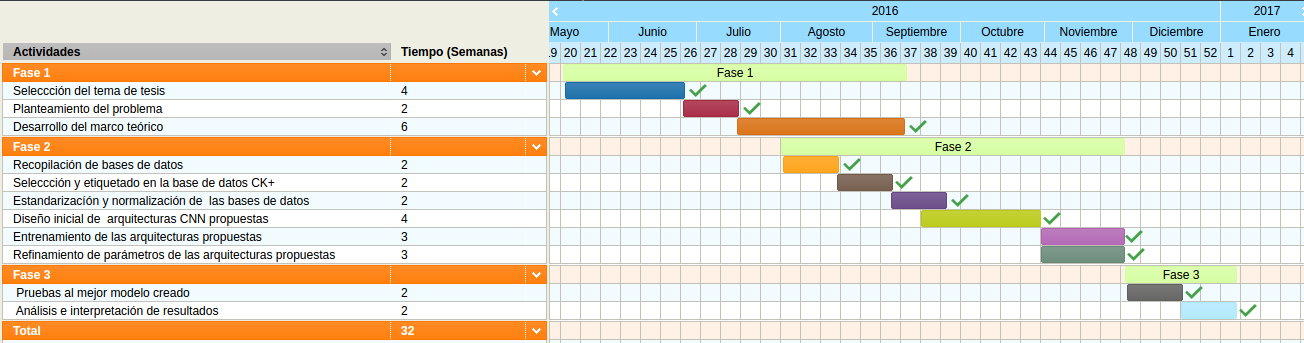
\includegraphics[angle=90,width=50mm]{Imagenes/cronograma.png}
    \caption{Cronograma de actividades}
    \label{tab:tab1}
\end{table}


 

\part{Marco Teórico}
\chapter{Marco Teórico}
\section{Conceptos de Visión}

\subsection{Visión Humana}
De una manera muy generar, vision se entiendo como toda accion de ver, sin embargo, desde un punto de vista mas tecnico, vision es la capacidad de interpretar nuestro entorno gracias a los rayos de luz que alcanzan el ojo. Otros autores definen vision como una capacidad necesaria mas no impresindible para realizar las actividades cotidianas.

Desde el punto de la vista de la medicina, la visión humana o sentido de la vista se reduce a un organo receptor conocido como el \textit{ojo}, la membrana y retina son los encargados de recivir las impresiones luminosas para luego transmitirlas al cerebro por medio de las vias opticas(ver figura~\ref{fig:estructura_percepcion}). En adicion, el ojo es un organo situado en la cavidad orbitaria, esta protegida por los parpados y por la secrecion de las glandulas lagrumales. Los ojos son sensibles a ondas de radiación electromagnética de longitudes específicas. Estas ondas se registran como la sensación de la luz. Cuando la luz penetra en el ojo, pasa a través de la córnea, la pupila y el cristalino, y llega por último a la retina, donde la energía electromagnética de la luz se convierte en impulsos nerviosos que pueden ser utilizados por el cerebro. Los impulsos abandonan el ojo a través del nervio
óptico. La región más sensible del ojo en la visión normal diurna es una pequeña depresión de la retina llamada fóvea en el cual se enfoca la luz que viene del centro del campo visual (por campo visual entendemos aquello a lo que mira el sujeto). Puesto que la lente simple convexa invierte la imagen, el campo visual derecho es representado a la izquierda de la retina y el campo inferior representado en lo alto de la retina. El ojo es un sistema óptico muy imperfecto. Las ondas de luz no solo tienen que pasar a través de los humores y el cristalino, después penetrar la red de los vasos sanguíneos y fibras nerviosas antes de que lleguen las células sensibles los bastones y los conos de la retina donde la luz se convierte en impulsos nerviosos. A pesar de estas imperfecciones el ojo funciona muy bien. La fóvea es capaz de percibir un cable telefónico a 400 m de distancia. En buenas condiciones el ojo puede percibir un alambre cuyo grosor no cubre más de 0,5 mm.

Tambien exister otras definiciones que indican que, el ojo es la puerta de entrada por la que ingresan los estímulos luminosos que se transforman en impulsos eléctricos gracias a unas células especializadas de la retina que son los conos y los bastones. Entonces, el nervio óptico transmite los impulsos eléctricos generados en la retina al cerebro, donde son procesados en la corteza visual. Finalmente, en el cerebro tiene lugar el complicado proceso de la percepción visual gracias al cual somos capaces de percibir la forma de los objetos, identificar distancias, detectar los colores y el movimiento~\cite{14alonso2005personas}.


        \begin{figure}[H]
		\centering
		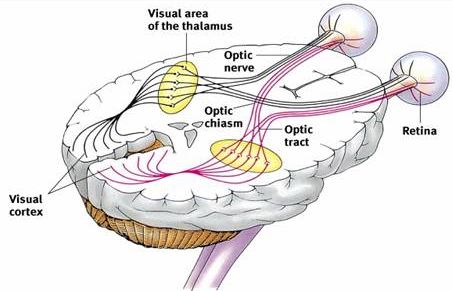
\includegraphics[width=120mm]{Imagenes/estructura_percepcion.jpg}
		\caption{Estructura de la percepción visual humana.}
		\vspace{0.15cm}
		\textit{Fuente: Fernando Vila Arroyo, “El Libro Blanco de la Iluminación”. España 2013.}
		\label{fig:estructura_percepcion}
		\end{figure}      	  

\subsection{Visión por Computador}
La visión artificial o también conocida como visión por computador es una disciplina científica que incluye métodos para adquirir, procesar, analizar y comprender las imágenes del mundo real con el fin de producir información numérica o simbólica para que puedan ser tratados por un computador. Tal y como los humanos usamos nuestros ojos y cerebros para comprender el mundo que nos rodea, la visión por computador trata de producir el mismo efecto para que las computadoras puedan percibir y comprender una imagen o secuencia de imágenes y actuar según convenga en una determinada situación. Esta comprensión se consigue gracias a distintos campos como la geometría, la estadística, la física y otras disciplinas. La adquisición de los datos se consigue por varios medios como secuencias de imágenes, vistas desde varias cámaras de video o datos multidimensionales desde un
escáner médico.

Hay muchas tecnologías que utilizan la visión por computador(figura~\ref{fig:esquema_vision_computador}), entre las cuáles tenemos: reconocimiento de objetos, detección de eventos, reconstrucción de una escena (\textit{mapping}) y restauración de imágenes~\cite{15VC}.


\begin{figure}[H]
		\centering
		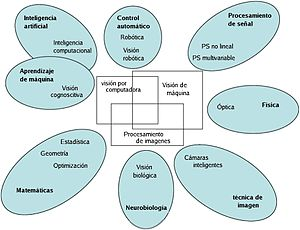
\includegraphics[width=100mm]{./Imagenes/esquema_vision_computador.jpg}
		\caption{Esquema de las relaciones entre la visión por computadora y otras áreas afines.}
		\vspace{0.15cm}
		\textit{Fuente: Visión artificial, Wikipedia.}
		\label{fig:esquema_vision_computador}
\end{figure}  


\section{Deteccion de Rostros}
En los ultimos años investigadores de todo el mundo vienen trabajando en la detección y reconocimiento de rostros, esto, debido a la gran cantidad de aplicaciones que este brinda, aplicaciones relacionadas con la seguridad publica, estudios de marketing y psicologia de las personas. El rostro es una de las partes del cuerpo que mas rasgos representativos muestra en una persona, por lo cual es de suma importancia poder identificar, reconocer y clasificar cada una de estas caracteristicas, de ahi su gran importancia para el desarrollo de las aplicaciones antes mencionadas. En la localización o deteccion de rostros, la primera etapa de los sistemas automatizados basados en visión por computador es encontrar el área que envuelve el rostro dentro de la imagen de entrada. La ubicación exacta de la cara es todavía una tarea difícil. Dentro de los muchos trabajos orientados a resolver este problema, Viola-Jones ha sido ampliamente utilizada debido a su robuste para la localizacion de objetos. La segunda etapa relacionada con el reconocimiento o clasificacion de rostros es otra tarea muy estudiada. En generar para realizar esta tarea son utilizados algoritmos de clasificacion de imagenes que estan disponibles en muchas librerias \textit{open source}, tales como OpenCV~\cite{20padilla2012evaluation}.

\subsection{Haar Cascade}
\label{sec:Haar_Cascade}
\textit{Haar Cascade} es un efectivo método para la deteccion de objetos, basado en la utilizacion de características de tipo \textit{Haar} este metodo resulta muy eficiente y robusto para este tipo de tareas. Fue propuesto por Paul Viola y Michael Jones, de ahí el sobrenombre Viola-Jones. Debido a que este método sirve para la deteccion de objetos, investigadores vieron por conveniente aprovechar sus grandes cualidades para la deteccion de rostros, alcanzando asi altos niveles de precisión en esta tarea. Existen muchas librerías \textit{open source} que disponibilizan modulos con la implementacion de este algoritmo, una de esas tantas es la popular librería \textit{Open Computer Vision Library} mas conocida como OpenCV, el \textit{framework} general de detectores de objetos se ha popularizado y ha motivado a la comunidad a generar sus propios clasificadores de objetos. Estos clasificadores usan características parecidas a las del tipo \textit{Haar} que se aplican sobre la imagen.~\cite{20padilla2012evaluation}.

\textit{Haar Cascade} de una manera resumida, es un enfoque basado en \textit{machine learning}, donde, una funcion \textit{cascade} es entrenada con muchas imagenes positivas(imagenes de caras) y negativas(imagenes que no sean caras). Entonces, se extraen las características de ellas, entrenando un modelo capaz de reconocer rostros con dichas caracteristicas.

\begin{figure}[H]
		\centering
		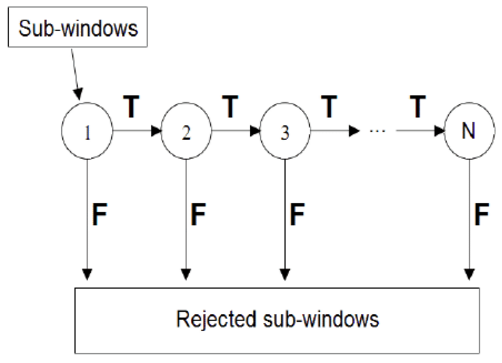
\includegraphics[width=80mm]{Imagenes/deteccion_cascade.png}
		\caption{Detección Cascade.}
		\vspace{0.15cm}
		\textit{Fuente: Evaluation of Haar Cascade Classifiers for Face Detection, OpenCV.}
		\label{fig:deteccion_cascade}
\end{figure} 

\section{Redes Neuronales}
\subsection{Biológicas}

Son el principal elemento del Sistema Nervioso. Las redes neuronales biológicas son el resultado de la union de varias neuronas entrelazadas entre si. Una neurona es una célula compuesta por tres partes fundamentales: el cuerpo, un numero de extensiones llamadas dendritas que sirven de entradas, y una larga extensión llamada axón, la cual se activa como salida. Existe un proceso de comunicacion entre neuronas, el cual es conocido como 'la sinapsis', este proceso conecta el axón de una neurona a las dendritas de las otras neuronas para comunicarse por medio de impulsos electricos. Las neuronas están dispuestas en multiples capas. Por lo general las neuronas de una primera capa reciben entradas desde otra capa y envían sus salidas o impulsos nerviosos a las neuronas de una tercera. Existe un proceso de retroalimentación que se origina cuando los impulsos nerviosos de una neuronal son enviadas a ella misma, originando asi un ciclo donde la imformacion se mantiene por periodos de tiempo. Similar, puede ocurrir la comunicacion entre neuronas de la misma capa.

Las conexiones entre neuronas tienen pesos asociados que representan la influencia de una sobre la otra. Si dos neuronas no están conectadas, el correspondiente peso de enlace es cero. Esencialmente, cada una envía su información de estado multiplicado por el correspondiente peso a todas las neuronas conectadas con ella. Luego
cada una, a su vez, suma los valores recibidos desde sus dendritas para actualizar sus estados respectivos.

Las redes biologicas son entrenadas por medio de la experiencia vivida durante el dia a dia (imagenes recolectadas por el ojo humana y procesadas por el cerebro), de esta forma, estimulando a cada neurona a aprender caracteristicas especiales que ayuden a identificar un determinado objeto. Cabe mencionar que la efectividad y precisión con la que se pueda reconocer un objeto, depende mucho de la cantidad de imagenes previas que se ayan visto sobre este. Además, se producirán respuestas cuando, en la utilización, se presenten entradas totalmente nuevas para el sistema. De este modo el sistema de red neuronal no reside necesariamente en la elegancia de la solución particular sino en su generalidad de hallar solución a problemas particulares, habiéndose proporcionado ejemplos del comportamiento deseado. Esto permite la evolución de los sistemas autómatas sin una reprogramación explicita~\cite{21RedesNeuronales}.

De acuerdo con estudios previos, muchos trabajos orientados al estudio del cerebro humano y la medicina, mencionan que una persona tiene alrededor de $10^{11}$ neuronas, cada una con alrededor de $10^4$ salidas. Donde, la estructura de neuronas de la corteza cerebral es modular: si bien todas las partes del cerebro son relativamente similares, diferentes partes hacen diferentes cosas; a partir de una estructura general, según la experiencia se generan nuevas estructuras especificas al problema a resolver~\cite{16pusiol2014redes}. 


\begin{figure}[H]
		\centering
		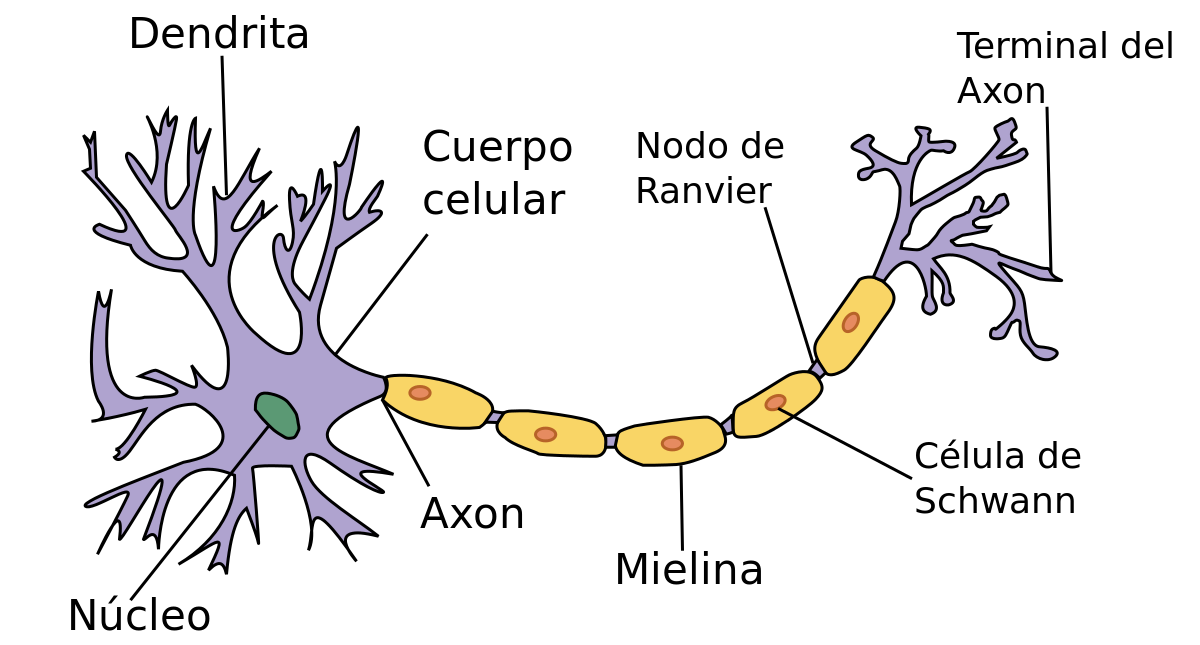
\includegraphics[width=100mm]{Imagenes/neurona_biologica.png}
		\caption{Neurona biológica}
		\vspace{0.15cm}
		\textit{Fuente: Patri Tezanos, Neurociencia, 2016.}
		\label{fig:neurona_biologica}
\end{figure} 


\subsection{Artificiales}
Las Redes Neuronales Artificiales (ANN) imitan el funcionamiento del cerebro, basicamente,  el tipo de  conexiones existentes (ejemplo: las neuronas de una capa previa estan conectadas a neuronas de la siguiente capa), estructura (numero de capas) y transferencia de informacion entre neuronas. Este tipo de arquitectura son aptas para resolver problemas que no poseen un algoritmo claramente definido, transformando asi una entrada en una salida; aprenden, reconocen y aplican relaciones entre objetos. Para realizar este tipo de procesos o tareas, se emplea normalmente un conjunto de ejemplos representativos para 'entrenar' el sistema o la red neuronal (en nuestro caso, imagenes de expresiones faciales), que, a su vez, se adaptan ajustando los pesos de cada neurona de tal manera que pueda producir salidas deseadas a cada imagen de entrada.

Además, similar a las redes neuronales biologicas, se producirán respuestas, cuando en la utilización se presenten entradas totalmente desconocidas por el sistema entrenado. De este modo el sistema de red neuronal artificial no se limita a solo reconocer imagenes que ayan sido previamente vistas, sino en su generalidad para hallar similaridades entre la imagen de entrada y las imagenes previas antes de la fase de entrenamiento, generando asi un sistema robusto capaz de obtener una semejansa enorme a las redes neuronales biologicas.

Las Redes Neuronales Artificiales se basan en el circuito de procesamiento de entradas en el cual los pesos son sumados. Las funciones de peso son conocidas generalmente como atenuadores. En la implementación, las entradas a una neurona son pesadas multiplicando el valor de la entrada por un factor que es menor o igual a uno. El valor de los factores de peso es determinado por el algoritmo de aprendizaje. Las entradas atenuadas son sumadas usando una función no lineal llamada 'Sigmoide'. Si la salida de la función suma excede el valor de entrada máximo de la neurona, esta responde generando una salida. Cada neurona tiene varias entradas y su salida está conectada a un conjunto de otros procesadores de entradas.

Cuando una red funciona en modo normal, a partir de los datos presentados en la entrada, se genera un patrón especifico de salida. La relación entre la entrada y la salida será determinada durante la etapa de  entrenamiento, entonces cuando una entrada conocida es presentada sera dada una salida efectiva. Durante esta etapa de entrenamiento, el algoritmo de aprendizaje ajusta los pesos de las entradas hasta que se alcanza la salida esperada, esto se logra por medio de la minimización de una función de costo(ver ecuación~\ref{eq:funcion_salida}), la cual es representada como la diferencia entre la salida esperada y la salida obtenida.

Devido a la compleja conexión que se realiza entre capas de la red, la complejidad con respecto a terminos computacionales y tiempo de ejecución, puede crecer de manera exponencial. Esto de debe a que cada neurona esta conectada a cientos de neuronas de la siguiente capa y cada neurona de esa siguiente capa realiza lo mismo. Por lo tanto mientras mas sea el numero de capas y neuronas, aparentemente, el sistema sera mejor, pero tambien sera mas complejo y dificil de entrenar.~\cite{21RedesNeuronales}.

La figura~\ref{fig:neurona_artificial} muestra las partes de una neurona artificial, la cual es similar a la estructura de una neurona biologica.

\begin{equation}\label{eq:funcion_salida}
Y_{i} = f(\sum W_{i,j}X{j} - \theta{i})
\end{equation}

\begin{figure}[H]
		\centering
		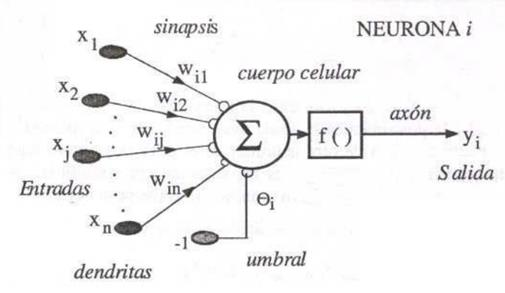
\includegraphics[width=100mm]{Imagenes/neurona_artificial.png}
		\caption{Modelo matemático de una red neuronal}
		\vspace{0.15cm}
		\textit{Fuente: Yuly Cristina Moreira Monserrate, Inteligencia Artificial, 2015.}
		\label{fig:neurona_artificial}
\end{figure}




\section{Arquitectura de una Red Neuronal Artificial}
\subsection{Capas}

\begin{figure}[H]
		\centering
		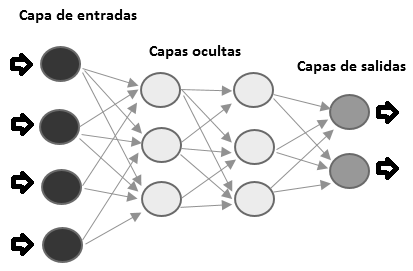
\includegraphics[width=100mm]{Imagenes/capas_red_neuronal.png}
		\caption{Capas de una red neuronal artificial.}
		\vspace{0.15cm}
		\textit{Fuente: Perceptrón multicapa, Wikipedia.}
		\label{fig:capa_red_neuronal}
\end{figure} 

Una red neuronal artificial esta compuesta por tres capas:
\begin{itemize}
\item \textbf{Capa de Entrada.- }Es la encargada de recepcionar los datos de entrada que posteriormente seran procesados. La representacion de estas estradas puede variar dependiendo del tipo de problema que se quiera resolver. En el aso de imagenes, esta se puede representar como una matriz que contiene un determinado valor representativo para cada pixel.
\item \textbf{Capa Oculta.- }Es la encargada de realizar el procesamiento pesado de la informacion, para posteriormente enviar la informacion ya procesada a la capa de salida.
información a la capa de salida.
\item \textbf{Capa de Salida.-} Contiene los resultados como una lista de números. Donde el numero de neuronas de la capa de salida tiene que ser igual al numero de posibles salidad que ofresca el problema a resolver. Otorgando un valor a cada neurona y finalmente, por medio de una funcion de normalizacion obtener la salida definitiva, que corresponde a una sola neurona.  
\end{itemize}


\subsection{Funciones de Activación}
La función de activación es la encargada de mantener los números producidos por cada neurona dentro de una rango razonable(generalmente números reales entre 0 y 1). Esta funcion recibe como entrada la suma de todos los números que llegan por medio de las conexiones entrantes, transforma el valor mediante una determinada funcion y produce un nuevo valor que sera utilizado para la siguiente iteracion. Existen distintas funciones de activacion estudiadas y experimentadas en trabajos previos, donde, algunas de ellas muestran mayor desempeño que las otras.

\begin{itemize}
\item \textbf{Función de activación Sigmoide}

Muchos procesos naturales y curvas de aprendizaje de sistemas complejos muestran una progresión temporal desde unos niveles bajos al inicio, hasta acercarse a un clímax transcurrido un cierto tiempo; la transición se produce en una región caracterizada por una fuerte aceleración intermedia. La función Sigmoide permite describir esta evolución. Su gráfica tiene una típica forma de "S" (ver figura~\ref{fig:funcion_sigmoid}), y esta limitada en el rango de 0 a 1 en el eje de las ordenadas. A menudo la función Sigmoide se refiere al caso particular de la función logística y que viene definida por la ecuación~\ref{eq:funcion_sigmoide}~\cite{24fsigmoide}.

\begin{equation}\label{eq:funcion_sigmoide}
f(x) = \frac{1}{1+\exp^{-x}}
\end{equation}

\begin{figure}[H]
		\centering
		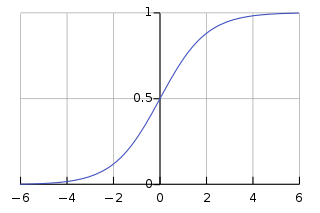
\includegraphics[width=90mm]{Imagenes/fSigmoid.png}
		\caption{Grafica de la función Sigmoide}
		\vspace{0.15cm}
		\textit{Fuente: Sigmoid Function, Wikipedia.}
		\label{fig:funcion_sigmoid}
\end{figure} 

\item \textbf{Función de activación Tangencial}

Es la versión continua de la función signo y se usa en problemas de aproximación. Es importante por sus propiedades analíticas. Es continua a valores en el intervalo [-1,1] (ver figura~\ref{fig:funcion_tang}) e infinitamente diferenciable, Esta función está definida esta definida por la ecuacion~\ref{eq:funcion_tanh}~\cite{25ftangencial}.

\begin{equation}\label{eq:funcion_tanh}
tanh(x) = \frac{\exp^x - \exp^{-x}}{\exp^x + \exp^{-x}}
\end{equation}

\begin{figure}[H]
		\centering
		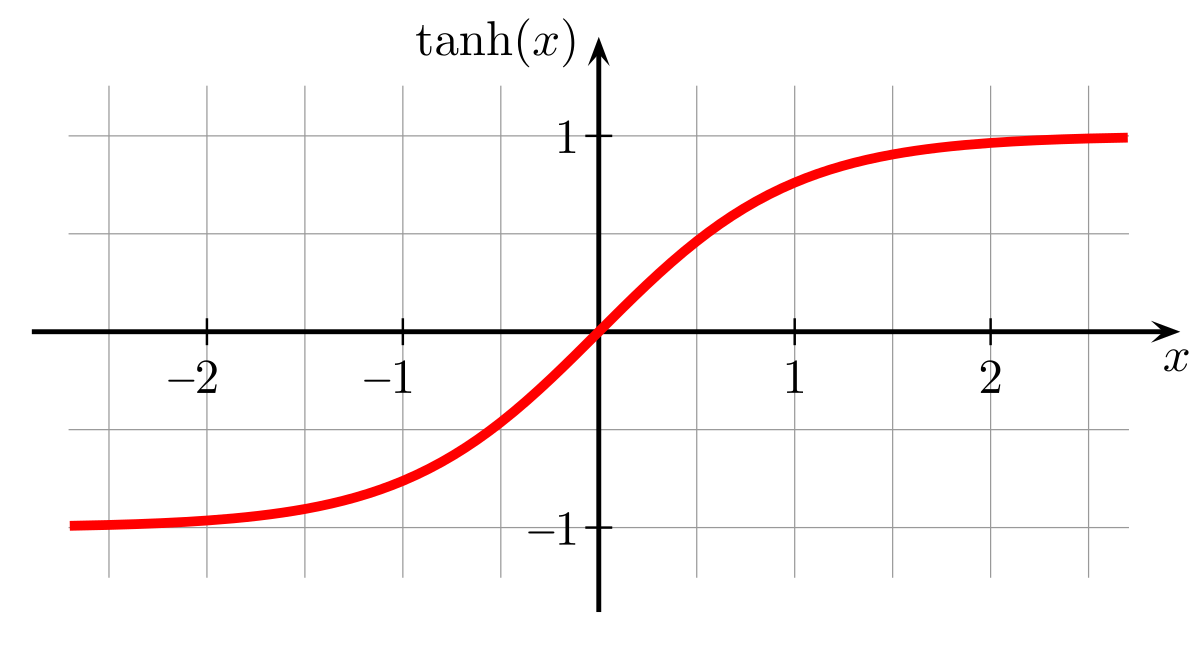
\includegraphics[width=90mm]{Imagenes/fTangent.png}
		\caption{Grafica de la función Tangencial}
		\vspace{0.15cm}
		\textit{Fuente: Tangente hiperbólica, Wikipedia.}
		\label{fig:funcion_tang}
\end{figure} 

\item \textbf{Función de activación RELU (\textit{Rectified Linear Unit})}

Se conoce como una función de rampa y es análoga a la rectificación de onda media. Esta función de activación fue introducida por primera vez a una red dinámica, en un artículo del año 2000, con fuertes motivaciones biológicas y justificaciones matemáticas. Finalmente en el año 2015, despues de ser usada dentro de las redes neuroanles convolucionales, alcanza un gran nivel de eficacia y robustes, superando ampliamente a las funciones de activación logística Sigmoide(la cual esta inspirada en la teoría de probabilidades) y tangente hiperbólica. Siendo asi la mas popular para las Redes Neuronales Profundas. Esta funcion es representada por medio de la ecuación~\ref{eq:funcion_Relu}, y debido a esa ecuación, la parte negativa en el eje abscisas se mantiene en cero, generando la grafica como se muestra en la figura~\ref{fig:funcion_relu}~\cite{26fRelu}.

\begin{equation}\label{eq:funcion_Relu}
f(x)=Max(0,x)
\end{equation}

\begin{figure}[H]
		\centering
		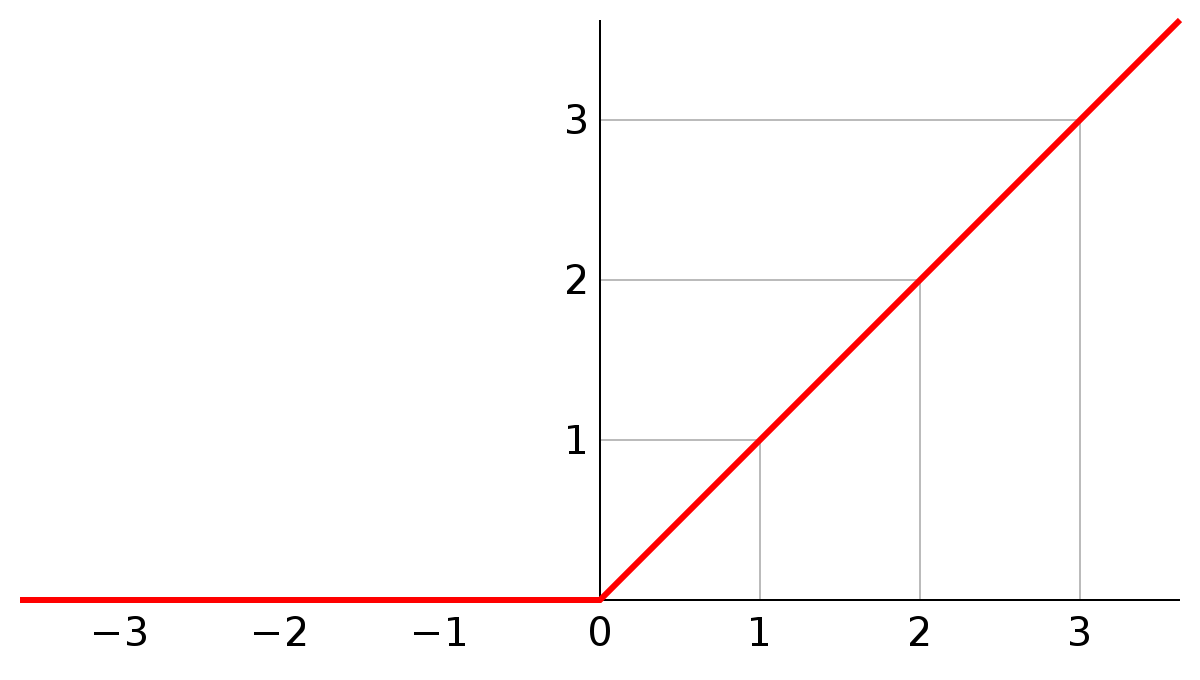
\includegraphics[width=90mm]{Imagenes/fRelu.png}
		\caption{Grafica de la función RELU}
		\vspace{0.15cm}
		\textit{Fuente: Hyperbolic tangent and ReLU neurons, Int8.}
		\label{fig:funcion_relu}
\end{figure} 

\end{itemize}
\subsection{Bias o Sesgo}
Es una cantidad constante que cada neurona de alguna capa oculta añade justo antes de aplicar la función de activacion, este valor puede incrementar o dismunir a la suma de productos(sumatoria de los productos obtenidos despues de multiplicar el valor de cada neurona con su respectivo peso que conecta hacia la siguiente neurona). El objetivo de este valor constante es lograr una convergencia más rápida de la red y evitar que el valor final entrante a una neurona sea un valor muy despreciable o muy significativo. La figura~\ref{fig:arquitectura_red_neuronal} muestra como este valor es intergado en la arquitectura de una red neuronal.


\begin{figure}[H]
		\centering
		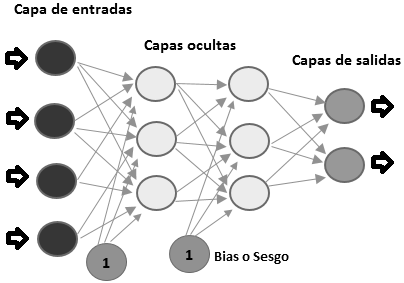
\includegraphics[width=100mm]{Imagenes/arquitectura_red_neuronal.png}
		\caption{Arquitectura de un RNA incluida el sesgo}
		\vspace{0.15cm}
		\textit{Fuente: Propio}
		\label{fig:arquitectura_red_neuronal}
\end{figure}

\section{Implementación de una Red Neuronal Artificial}
Una forma sencilla de implementar redes neuronales, consiste en almacenar los pesos en matrices. Se considera que la red neuronal es un grafo y simplemente representamos este grafo por medio de su matriz de adjacencia, donde cada posicion $(i,j)$ almacena el peso entre la neurona $i$ y la neurona $j$. Posteriormente guardamos los valores de todas las neuronas de una determinada capa en un vector, el producto del vector y la matriz de pesos de salida nos da los valores de entrada de cada neurona en la siguiente capa. Después se aplica la función de activación a cada elemento de ese segundo vector, y repetimos el proceso~\cite{21RedesNeuronales}.

La implementación antes mencionada es una idea general de como se podria implementar una red neuronal(no es el unico algoritmo). En la vida real existen distintos tipos de redes neuronales, donde cada una de ellas presenta una implementación diferente, siendo algunas de ellas mas eficientes computacionalmente que otras.

\section{Backpropagation}
\label{sub:backpropagation}
El \textit{BackPropagation} es un algoritmo de aprendizaje supervisado que se usa para entrenar redes neuronales artificial, dicho algoritmo se basa en el descenso de gradiente que es un algoritmo de optimización utilizado para determinar los valores de los parámetros (coeficientes) de una función $f$ que minimiza una función de costes. El descenso de gradiente se utiliza mejor cuando los parámetros no pueden ser calculados analíticamente (por ejemplo, usando algebra lineal) y deben ser buscados por un algoritmo de optimización~\cite{27lehr1993backpropagation}.

La figura~\ref{fig:back_propagation} muestra la representación de como el descenso de gradiente trabaja en la busqueda de los mejores parametros para una determinada funcion (ejemplo: sea la function $f(x)=ax+b$, donde los parametros son las constantes $a$ y $b$). El objetivo es alcanzar el circulo central, el cual representa los parametros óptimos buscados. Para alcanzar dicho objetivo se realiza una serie de paso (representados por las rectas trazadas entre cada par de puntos rojos, como se muestra en la figura~\ref{fig:back_propagation}) que sirven para ajustar los parametros de tal forma que poco a poco se acerquen a la funcion objetivo.

El algoritmo de \textit{Backpropagation} es muy intuitivo. Dada una entrada a la red, esta genera una salida, la cual posteriormente es comparada con la salida deseada, consiguiendo asi el primer error de salida (funcion de costo o diferencia entre la salida deseada y la salida obtenida por la red). Seguido, este error es propagado hacia atras, distribuyendo una porcion de dicho error a todas las neuronas de la capa anterior que aportaron para la obtención de la salida alcanzada. Este proceso se repite, capa por capa, hasta que todas las neuronas de la red ayan recibido una porcion del error obtenido. El objetivo de realizar estos pasos, es crear una red cuyos pesos de cada neurona minimizen la funcion de costo, consiguiendo asi un nivel de precision inversamente proporcional al error alcanzado por cada entrada(mientras menos error, mayor sera la precision alcanzada).

Matematicamente, el descenso de gradiente esta basado en la observación de que si la funcion multivariable $F(x)$ es definida y  diferenciable en la vecindad del punto $a$, entonces $F(x)$ decrece rapidamente si uno de ellos va desde $a$ en dirección del gradiente negativo de $F$ (donde la gradiente negativa esta representada por $-\bigtriangledown F(a)$). Se deduce que si, $a_{n+1} = a_n - \gamma \bigtriangledown F(a)$, para un $\gamma$ suficientemente pequeño, entonces $F(a_n)\geq F(a_{n+1})$. En otras palabras, el termino $\gamma \bigtriangledown F(a)$ es substraido desde $a$ porque se quiere mover a travez de la gradiente.  Con esta observación en mente,  se comienza con la suposición $x_0$ para un mínimo local de $F$, y se considera la secuencia $X_0, X_1, X_2,...$, tal que: $x_{n+1} = x_n - \gamma_n \bigtriangledown F(x_n), n\geq0$. Entonces nosotros tendremos $F(x_0)\geq F(x_1) \geq F(x2) \geq ...$ esperando que la secuencia converga en el mínimo local esperado. Se debe tener en cuenta que el valor del tamaño del paso $\gamma$ puede cambiar en cada iteración, obteniendo así la siguiente ecuación.

\begin{equation}
\gamma_n=\frac{(x_n - x_{n-1})^T [\bigtriangledown F(x_n)-\bigtriangledown F(x_{n-1})]}{||\bigtriangledown F(x_n)-\bigtriangledown F(x_{n-1})||^2}
\end{equation}
\begin{figure}[H]
		\centering
		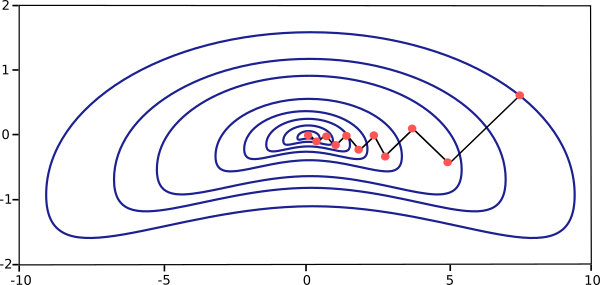
\includegraphics[width=80mm]{Imagenes/back_propagation.png}
		\caption{Descenso de gradiente.}
		\vspace{0.15cm}
		\textit{Fuente: 5 algorithms to train a neural network, Neural Designer.}
		\label{fig:back_propagation}
\end{figure}


\section{Deep Learning}
\label{sec:deep-learning}
El \textit{Deep Learning} es un concepto muy amplio, lo que implica que este tenga muchas definiciones. Sin embargo, de una forma muy general, se puede decir que el \textit{Deep Learning} es un concepto que surge de la idea de imitar el cerebro humano por medio de una abstracción mas profunda de las redes neuronales, con el objetivo de crear una inteligencia que mas se asemeje a la inteligencia humana, esta enfoque utiliza una capacidad de abstracción jerárquica, es decir, una representación de los datos de entrada en varios 'niveles'. A diferencia de las Redes Neuronales tradicionales, el \textit{Deep Learning} utiliza multiples capas ocultas para la selección de catacterísticas que son útiles para un mejor aprendizaje; de esta manera, la capa mas profunda dentro de las capas ocultas, obtendrán la representación de características con mayor nivel de abstracción(reconocimiento de lineas, puntos, curvas y otros).

Este enfoque no es mas que un conjunto de algoritmos de \textit{Machine Learning}, que intenta detectar abstracciones de un alto nivel en datos, haciendo uso de arquitecturas compuestas de transformaciones no-lineares multiples~\cite{17bengio2013representation}. Existen varios tipos de aprendizajes, las cuales son tomadas como base para el entrenamiento de una red neuronal en general. Sin embargo, dos principales categorías son resaltadas por las arquitecturas profundas (como se muestra en la figura~\ref{fig:aprendizajes}):

\begin{figure}[H]
		\centering
		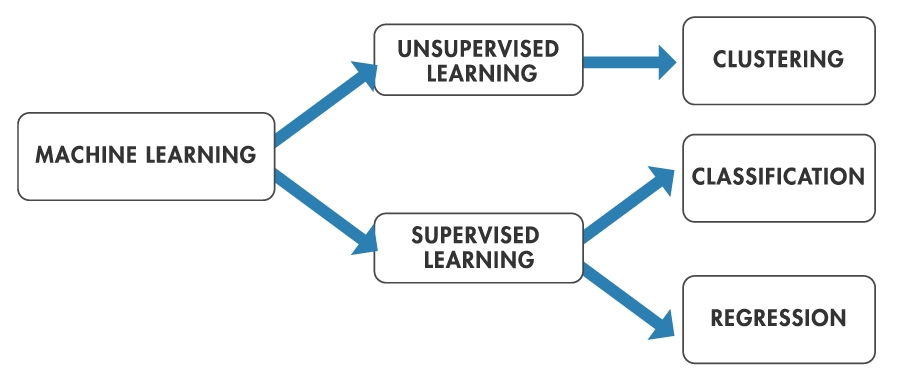
\includegraphics[width=130mm]{Imagenes/aprendizaje_tipos.jpg}
		\caption{Tipos de aprendizaje.}
		\vspace{0.15cm}
		\textit{Fuente: Big Data with MATLAB, Math Works.}
		\label{fig:aprendizajes}
\end{figure}

\begin{itemize}
\item \textbf{Supervisado: } Se caracteriza porque su entrenamiento es controlado por un agente
externo. Es decir, este agente externo guia el entrenamiento de la red mediante una comparacion entra la salida esperada y la salida obtenida por medio de la red. En otras palabras, para realizar este proceso, la base de datos a entrenar necesita contener un campo que indique la salida que se espera por cada dato de entrada. Por ejemplo, sea una arquitectura dedicada a la reconocimiento y clasificacion de numeros en imagenes, entonces, cada vez que pasemos una imagen como entrada a la red, esta imagen debera ir acompañada de una etiqueta que indique cual es el numero que se esta pasando~\cite{18restrepo2015aplicacion}.

\begin{figure}[H]
		\centering
		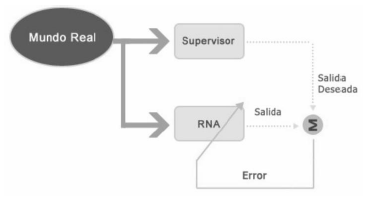
\includegraphics[width=75mm]{Imagenes/grafico_supervisado.png}
		\caption{Aprendizaje supervisado.}
		\vspace{0.15cm}
		\textit{Fuente: López S, Jesús A. Caicedo B, Eduardo F.}
		\label{fig:grafico_supervisado}
\end{figure}



\item \textbf{No supervisado: }
Este enfoque sugiere que el aprendizaje sea realizado presentándole a la red los datos directamente, es decir, ahora no existe un agente externo, campo o etiqueta que indique a la red cuales son los datos que se le proporciona como entrada. La red aprende de ellos, agrupandolos de acuerdo a la similaridad de sus caracteristicas, en algunos casos se realiza este tipo de agrupacion de forma probabilística~\cite{18restrepo2015aplicacion}.

\begin{figure}[H]
		\centering
		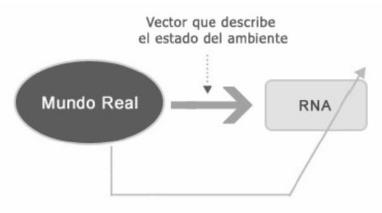
\includegraphics[width=75mm]{Imagenes/grafico_no_supervisado.png}
		\caption{Aprendizaje no supervisado.}
		\vspace{0.15cm}
		\textit{Fuente: López S, Jesús A. Caicedo B, Eduardo F.}
		\label{fig:grafico_no_supervisado}
\end{figure}

\item \textbf{Híbrido: }
Algunas redes tienden a utilizar ambos tipos de aprendizaje para su fase de entrenamiento, ya sea comenzando por un pre-entrenamiento supervisado y finalizando con uno no supervisado o viceversa. Este enfoque se sigue con el objetivo de logran un mejor ajuste, disminuyendo el tiempo de convergencia y entre otras funcionalidades~\cite{18restrepo2015aplicacion}.
\end{itemize}

\section{Redes mas Comunes Consideradas dentro del Deep Learning}
\subsection{Autoencoder}
Es un tipo de Red Neuronal Artificial utilizada para el aprendizaje no supervisado de codificaciones eficientes. El objetivo de una autoencoder es aprender una representación (codificación) para un conjunto de datos, típicamente con el propósito de reducción de dimensionalidad. Recientemente, el concepto autoencoder se ha vuelto más ampliamente utilizado para el aprendizaje de modelos generativos de datos~\cite{28fAutoencoder}.

Un auto-codificador, o autoencoder, aprende a producir a la salida exactamente la misma información que recibe a la entrada. Por eso, las capas de entrada y salida siempre deben tener el mismo número de neuronas. Por ejemplo, como se muestra en la figura~\ref{fig:autoencoder}, si la capa de entrada recibe los píxeles de una imagen, se espera que la red aprenda a producir en su capa de salida exactamente la misma imagen que ha sido introducido~\cite{18restrepo2015aplicacion}.

\begin{figure}[H]
		\centering
		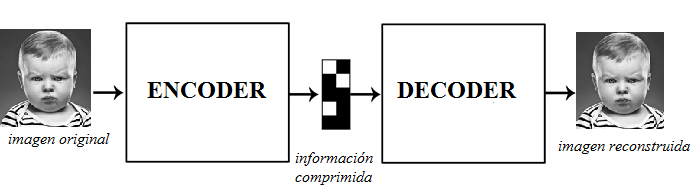
\includegraphics[width=150mm]{Imagenes/autoenconder.png}
		\caption{Arquitectura de una red neuronal Auto-encoder.}
		\vspace{0.15cm}
		\textit{Fuente: Propio.}
		\label{fig:autoencoder}
\end{figure}

\subsection{Redes Neuronales Recurrentes}
Las Redes de Neuronas Recurrentes (\textit{Recurrent Neural Networks}) no tienen una estructura de capas definida, sino que permiten conexiones arbitrarias entre todas las neuronas, incluso creando ciclos. Esto permite incorporar a la red el concepto de temporalidad, y permite que la red tenga memoria, porque los números que introducimos en un momento dado en las neuronas de entrada son transformados, y continúan circulando por la red incluso después de cambiar los números de entrada por otros diferentes~\cite{18restrepo2015aplicacion}.

Este tipo de redes, debido a la capacidad de retener informacion por cortos periodos de tiempo, es altamente utilizado en trabajos relacionados con el procesamiento y analisis de videos, donde las entradas a la red son un conjunto de frames(imagenes), siendo cada imagen la continuacion de la anterior. Sin embargo, similar a las otras redes neuronales, la complejidad en teminos de tiempo de ejecucion(entrenamiendo de la red) sigue siendo una limitacion para experimentar con dichos trabajos, ya que el numero de parametros a optimizar siguen siendo miles de miles, debido a las multiples conexiones que se presentan entre neuronas.  


\begin{figure}[H]
		\centering
		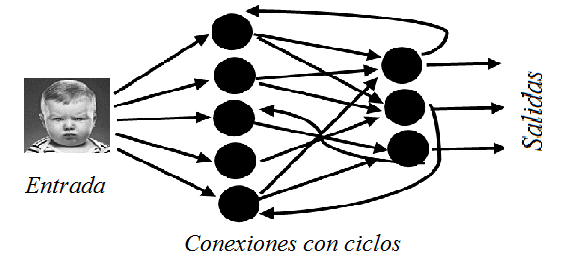
\includegraphics[width=130mm]{Imagenes/red_recurrente.png}
		\caption{Arquitectura de una red neuronal Recurrente.}
		\vspace{0.15cm}
		\textit{Fuente: Propio.}
		\label{fig:red_recurrente}
\end{figure}

\subsection{Redes Neuronales Convolucionales}
Las Redes Neuronales Convolucionales (\textit{Convolution Neural Network}) a diferencia de las Redes Neuronales Recurrentes, mantienen el concepto de capas, pero cada neurona de una capa no recibe conexiones entrantes de todas las neuronas de la capa anterior, sino sólo de algunas. Esto favorece que una neurona se especialice en una región de la lista de números de la capa anterior, y reduce drásticamente el número de pesos y de multiplicaciones necesarias. Lo habitual es que dos neuronas consecutivas de una capa intermedia se especialicen en regiones solapadas de la capa anterior~\cite{16pusiol2014redes}.

Muy diferente del esquema tradicional de las Redes Neuronales Artificiales, estas redes presentan una gran variedad de tipos de capas, donde cada una de ellas tiene una función específica y esta puede repetirse mas de una vez. La siguiente sección sera dedicada a describir con mayor detalles la arquitectura modelo de una Red Neuronal Convolucional.

\section{Arquitectura de una Red Neuronal Convolucional}

Las Redes Neuronales Convolucionales son una estructura compuesta de varias fases entrenables, aprendiendo de cada una de las características con diferentes grados de abstracción. La entrada y salida de cada una de estas etapas son conjunto de arreglos llamados mapas de características, a la salida cada mapa de características representa una característica particular extraída de la imagen de entrada. Cada fase generalmente está compuesta por tres capas: Convolucion, función no lineal y una capa de sub-muestreo. Las ultimas capas por lo general son un conjunto de capas totalmente conectadas.

Una típica arquitectura de Red Neuronal Convolucional para clasificación supervisada está basada en varias etapas(los tres tipos de capas mencionadas en el parrafo anterior: Convolucion y sub-muestreo) seguidas de un clasificador(el conjunto de capas totalmente conectadas). Una de las primeras arquitecturas, es la red propuesta por Yann LeCun(figura~\ref{fig:arquitectura_CNN_Lecun}). Esta red fue utilizada para resolver el problema de reconocimiento de caracteres manuscritos, utilizando una arquitectura con dos fases.


\begin{figure}[H]
		\centering
		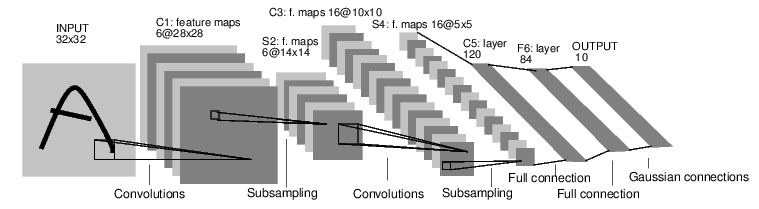
\includegraphics[width=160mm]{Imagenes/arquitectura_CNN_Lecun.png}
		\caption{Arquitectura de una red neuronal Convolucional.}
		\vspace{0.15cm}
		\textit{Fuente: Source: Yann LeCun, 1998.}
		\label{fig:arquitectura_CNN_Lecun}
\end{figure}

Esta red denominada Let-Net, toma una imagen como entrada, la capa siguiente esta constituido por un conjunto de filtros de convolución (mapas de características), seguida por una capa de sub-muestreo encargada de la reduccion de dimensionalidad, seleccionando asi solo los datos mas relevantes. La capa de convolución esta compuesta por seis mapas de características, donde cada uno de ellos no es mas que una matriz con valores asociados. A continuación, se encuentra la capa de sub-muestreo, que, como se menciono antes, agrupa las salidas de las nuevas imágenes originadas por la capa de convolución, generando asi la misma imagen pero con dimensiones menores e información mas relevante. Este nuevo mapa de características sirve de entrada para la siguiente fase dedicada a encontrar características de mayor abstracción. Una cosa importante que cabe resaltar, es que, a medida que se avanza en las fases se aprenden caracteristicas mas relevantes, pero mas invariantes a posicion(por el sub-muestreo). Finalmente, las capas totalmente conectadas se encargan de evaluar las posibles combinaciones de las características aprendidas para lograr clasificar las imágenes dadas~\cite{16pusiol2014redes}.

\subsection{Capa de Convolución}
La capa de convolución es el bloque de construcción básico de una red, esta capa hace la mayor parte del trabajo pesado computacional, debido a que se realizan multiplicaciones de matrices entre la imagen y los filtros de convolución.
\begin{itemize}
\item \textbf{Visión general e intuición sin cerebro.} Los parametros de la capa de convolución consisten en un conjunto de filtros que durante la fase de entrenamiento son aprendidos. Cada filtro es pequeño espacialmente (a lo largo de la anchura y altura), este filtro es aplicado a través de toda la imagen de entrada. Por ejemplo, un filtro típico en una primera capa de una Red Neuronal Convolucional podría tener un tamaño de 5x5x3 (es decir, 5 píxeles anchura y la altura, y 3 ya que las imágenes tienen profundidad 3, los canales de color). Durante el la operacion de convolucion entre el filtro y la imagen de entrada, este se desliza a través del ancho y la altura del volumen de entrada y calcula el productos escalares entre estos dos elementos. A medida que se desplaza el filtro sobre la anchura y la altura del volumen de entrada se produce un mapa de activación de 2 dimensiones que da las respuestas de ese filtro en cada posición espacial. Intuitivamente, la red aprenderá filtros que se activan cuando ven algún tipo de función visual, como un borde en una determinada orientación o una mancha de un cierto color. Después se tendrá todo un conjunto de filtros en cada capa de convolución, y cada uno de ellos va a producir un mapa de activación de 2 dimensiones por separado. Finalmente se apilan estos mapas de activación a lo largo de la dimensión de la profundidad y producen el volumen de salida.~\cite{22RedesNeuronalesConvolu}.

\item \textbf{La vista del cerebro.} Cada entrada en el volumen de salida 3D también se puede interpretar como una salida de una neurona que mira sólo una pequeña región en los parámetros de entrada y comparte con todas las neuronas de la izquierda y derecha (ya que todos estos números resultaría de aplicar el mismo filtro).~\cite{22RedesNeuronalesConvolu}.

\item \textbf{Conectividad local.} Cuando se trata de entradas de alta dimensión como las imágenes, como se vio anteriormente, no es práctico conectar neuronas a todas las neuronas en la capa anterior. En su lugar, se va a conectar cada neurona a sólo una región local del volumen de entrada. La extensión espacial de esta
conectividad es un hiperparámetro llamado campo receptivo de la neurona (equivalente al tamaño del filtro). La extensión de la conectividad a lo largo del eje de profundidad es siempre igual a la profundidad del volumen de entrada. Es importante destacar nuevamente esta asimetría en cómo tratamos las dimensiones espaciales (anchura y altura) y la dimensión de la profundidad: Las conexiones son locales en el espacio (a lo largo del ancho y la altura), pero siempre llenas a lo largo de toda la profundidad del volumen de entrada~\cite{22RedesNeuronalesConvolu}.


\begin{figure}[H]
		\centering
		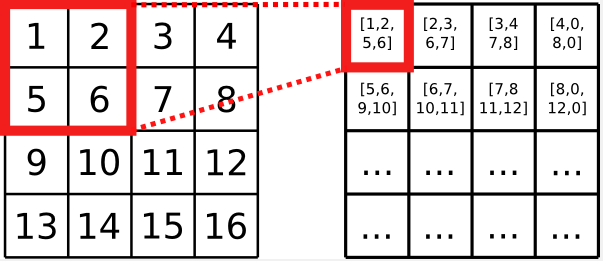
\includegraphics[width=100mm]{./Imagenes/convolucion.png}
		\caption{Ejemplo de convolución con un filtro de dimensiones de 2$\times$2.}
		\vspace{0.15cm}
		\textit{Fuente: Que es y como funciona Deep Learning, Rubén López.}
        	\label{fig:convolucion}
\end{figure}


\item { \textbf{Pseudo – Codigo.} La representacion de la convolucion por medio de una formula matematica se muestra en la ecuacion~\ref{eq:ecuac_conv}. Los valores de un píxel en la imagen de salida se calculan multiplicando cada valor del kernel por los valores de píxeles de la imagen de entrada correspondientes. Esto se puede describir algorítmicamente con el siguiente pseudo-código:

\begin{equation}\label{eq:ecuac_conv}
V = \frac{\sum^{q1}_{i=0}\sum^{q2}_{i=j} f_{i,j}*k_{i,j}}{F}
\end{equation}

\begin{algorithm}
\caption{Pseudo-Codigo Convolucion\\
La convolucion de una image f(x,y) con un kernel k(x,y) con dimensiones h$\times$w y (2h+1)$\times$(2w+1) respectivamente produce una nueva imagen g(x,y)}\label{alg:euclid}
\begin{algorithmic}[H]
\Procedure{Convolucion}{$f,k$}\Comment{Convolucion de la imagen f con el kernel k}

\For{\texttt{y:=1 to W}}

\For{\texttt{x:=1 to H}}
  \State $sum=0$
     \For{\texttt{i:=-h to h}}
		\For{\texttt{j:=-w to w}}
           \State $sum=sum + k(j,i)*f(x-j,y-i)$
		\EndFor
	 \EndFor 
  \State $g(x,y)=sum$
\EndFor
\EndFor
\State \textbf{return} $g$\Comment{Resultado de la convolucion entre f y k}
\EndProcedure
\end{algorithmic}
\end{algorithm}

Donde:
\begin{itemize}
\item $f_{i,j}$: Corresponde al pixel en la posición $i,j$ de la imagen f respecto al kernel k.
\item $k_{i,j}$: Corresponde al pixel en la posición $i,j$ del kernel k.
\item $q1\times q2 = (2h+1)\times(2w+1)$: Representa las dimensiones del kernel.
\item $F$: Es la suma de los coeficientes del kernel (1 si la suma es igual a 0).
\item $g(i,j)$: Representa el valor de salida del pixel en la posición $i,j$.
\end{itemize}}

\end{itemize}
first revision and fix of the theoretical framework

\subsection{Submuestreo}
La arquitectura tradicional de una red neuronal convolucional sugiere que se inserte una capa de sub-muestreo despues de cada capa de convolucion. Su función es reducir progresivamente el tamaño espacial de la imagen de entrada con el objetivo de reducir la cantidad de parámetros a ser calculados en la red, y por lo tanto, también para controlar el sobre ajuste. La capa de agrupación funciona independientemente en cada segmento de profundidad de la entrada y la redimensiona espacialmente, dependiende de las dimensiones de la ventana de sub-muestre. Existen diferentes funciones de agrupación para realizar este tipo de operacion, funciones como: MAX, MIN, MODA, MEDIANA, etc, cada una de estas funciones se desenvuelve de manera muy diferente, dependiendo del problema que ese pretende resolver. La forma más común es una capa de agrupación con filtros de tamaño 2x2 y función de agrupación MAX, aplicando un salto de dos pixeles hacia abajo y hacia arriba para realizar el desplazamiento e iterar la operacion de sub-muestreo sobre toda la imagen, de esta forma descartando el 75\% de las activaciones. En este caso, cada operación MAX tomaría un máximo de 4 números (pequeña región de dimensiones de 2x2). La dimensión de profundidad no cambia. Más generalmente, la capa de agrupación tiene estas principales características:

\begin{itemize}
\item Acepta un volumen de tamaño $W1\times H1\times D1$
\item Requiere 2 hiperparámetro
  \begin{itemize}
  \item Su extensión espacial $F$
  \item El desplazamiento $S$
  \end{itemize}
\item Produce un volumen de tamaño: $W2\times H2\times D2$, donde :
  \begin{itemize}
  \item $W2 =  \frac{W1 - F}{S + 1}$
  \item $H2 = \frac{H1 - F}{S + 1}$
  
  \item D2 = D1
  \end{itemize}
\item Introduce parámetros cero, ya que calcula una función fija de la entrada.
\item Tener en cuenta que no es común utilizar cero como relleno(\textit{padding}) para agrupar capas.
\end{itemize}

En la practica solo fueron encontradas dos variaciones comunes de la capa de sub-muestreo con función de agrupación MAX: Una capa de agrupación con F = 3, S = 2F, S = 2 (también llamada superposición de agrupación) y más comúnmente F = 2, S = 2F, S = 2. Los tamaños de agrupación con campos receptivos más grandes son demasiado destructivos~\cite{22RedesNeuronalesConvolu}.

\begin{figure}[H]
		\centering
		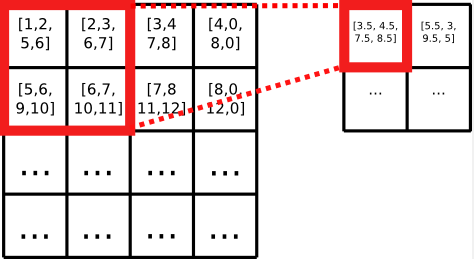
\includegraphics[width=100mm]{./Imagenes/submuestre.png}
		\caption{Ejemplo de Submuestreo con una ventana de 2X2 y calculando el promedio}
		\vspace{0.15cm}
		\textit{Fuente: Que es y como funciona Deep Learning, Rubén López.}
        \label{fig:submuestre}
\end{figure}


\subsection{Capa de normalización}
Existen muchos tipos de capas de normalizacion propuestas hasta la actualidad, algunos de ellos fueron creados con la intension de asemejar mas la red, al comportamiento real del cerebro. Sin embargo, estas capas a pesar de aparentar ser un gran aporte para conseguir una inteligencia artificial pura, han caido debido a que en la practica su aporte es casi nula. 

El objetivo de una capa de normalizacin es, como su mismo nombre lo dice, normalizar las activaciones de la capa anterior, es decir, se aplica una transformación que mantiene la activación de cierre media en 0 y la desviación estándar cerca de 1~\cite{22RedesNeuronalesConvolu}.

\subsection{Capa totalmente conectada}
Las neuronas en una capa completamente conectada tienen conexiones completas con todas las activaciones(neuronas) en la capa anterior, haciendo de este tipo de capas un grafo muy denso o grafo completo(figura~\ref{fig:grafico_full_conect}), el cual computacionalmente es muy costoso, sin embargo, generalmente dentro de las redes neuronales convolucionales, a lo mucho son usadas 2 a 3 capas totalmente conectadas, haciendo de este un trabajo ligeramente mas facil de computar. Este tipo de capas son como las que se ven en las redes neuronales regulares. Por tanto, sus activaciones pueden calcularse con una multiplicación matricial.~\cite{22RedesNeuronalesConvolu}.

Esta capa basicamente toma un volumen como entrada y su salida es un vector de N dimensiones, donde N es el número de clases correspondientes al problema que se esta resolviendo(en el caso de clasificación). Por ejemplo, si se esta trabajando en una red, la cual sera capaz de reconocer dígitos a partir de imágenes como entrada, entonces, el número de salidas sera 10(una salida para cada números del 0 a 9). Cada número en este vector de N dimensiones representa la probabilidad que este tiene para pertenecer a una determinada clase(esta probabilidad es obtenida gracias a la función de normalizacion, la cual se describe en la sub-sección~\ref{sub:softmax}), donde la suma de todas las probabilidades es 1. Sea el problema antes planteado, si el vector resultante es $[0, 0.1, 0.05 , 0.05, 0, 0, 0, 0, 0, 0.8]$, la probabilidad de que la imagen sea un 1 es de $10$\%, mientras que la probabilidad de que sea un 9 es de $80$\%.


\begin{figure}[H]
		\centering
		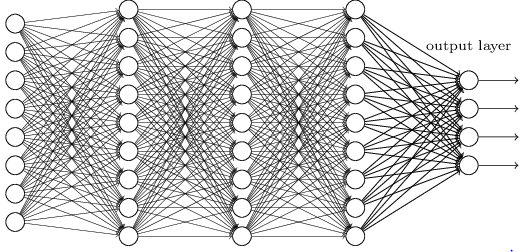
\includegraphics[width=120mm]{Imagenes/grafico_full_conect.png}
		\caption{Capa totalmente conectada}
		\vspace{0.15cm}
		\textit{Fuente: Michael A. Nielsen, http://neuralnetworksanddeeplearning.com/chap6.html}
		\label{fig:grafico_full_conect}
\end{figure}

\subsection{Función de normalización(Softmax)}
\label{sub:softmax}
La función de normalizacion softmax, tambien conocida como función exponencial normalizada, no es mas que nombre para la regresión lineal multinomial o simplemente clase múltiple de regresión logística. En su esencia, regresión de softmax es una generalización de la regresión logística que podemos utilizar para la clasificación de clase múltiple (bajo el supuesto de que las clases son mutuamente excluyentes). En cambio, utilizamos el modelo de regresión logística (estándar) en tareas de clasificación binario. 

Esta funcion tiene como entrada el vector de N dimensiones obtenida por la capa totalmente conectada, y como salida, un vector de probabilidades. La figura~\ref{fig:arquitectura_cnn_softmax} muestra como esta función se integra en la red. 

\begin{figure}[H]
		\centering
		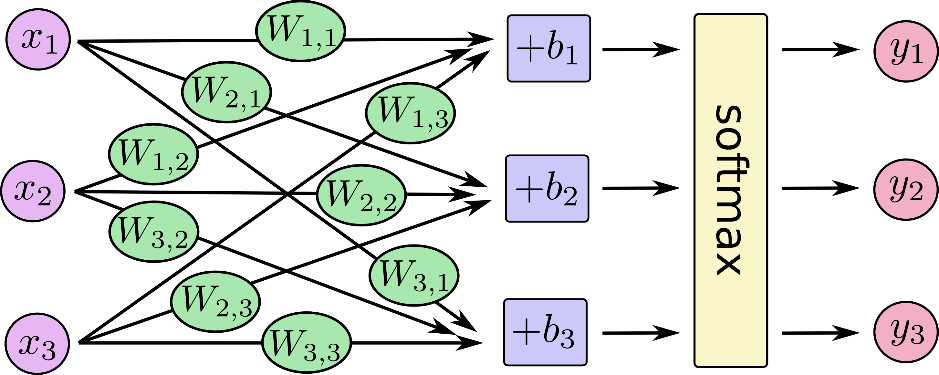
\includegraphics[width=120mm]{Imagenes/arquitectura_cnn_softmax.png}
		\caption{Arquitectura de una CNN con Softmax}
		\vspace{0.15cm}
		\textit{Fuente: Samuel Salvatella, http://ssalva.bitballoon.com/blog/2016-08-30-tensorflow/}
		\label{fig:arquitectura_cnn_softmax}
\end{figure}


En su representacion matematica, como se menciono antes, esta función es una generalización de la función logística que permite la utilización de un vector de dimensión. La función está dada por la ecuacion~\ref{eq:ecuac_soft}.

\begin{equation}\label{eq:ecuac_soft}
P(Y = j|Z^i) = \phi_{softmax}(Z^i)= \frac{\exp^{Z^i}}{\sum^k_{j=0}\exp^{Z^{i}_k}}
\end{equation}
Donde:

\begin{center} $Z = w_{0}x_{0} + w_{1}x_{1} +...+w_{m}x_{m} = \sum_{l=0}^m w_{l}x_{l} = w^Tx$\end{center}


\section{Entrenamiento de una Red Convolucional}

El proceso de entrenamiento en un red neuronal convoluciona, se basa en el algoritmo \textit{BackPropagation} (como se describió en la subsection~\ref{sub:backpropagation}), el cual consiste en calcular una función objetivo que minimiza el error, por medio de la retro propagación de este, hacia las capas anteriores, de tal manera que los pesos de las conexiones entre neuronas son ajustadas.

El algoritmo \textit{BackPropagation}, como se describio anteriormente, es muy intuitivo. Este sigue la siguiente secuencia de pasos:

\begin{itemize}
\item Primero, se proporciona datos de entrada a la red.
\item Segundo, son propagadas dichas entradas hasta la capa de salida, con pesos iniciales definidos o
aleatorios.
\item Tercero, se calcula el error en la capa de salida.
\item Cuarto, se propaga dicho error hacia las neuronas ocultas (hacia atrás).
\item Quinto, se cambia los pesos de las conexiones.
\end{itemize}

\section{Sobre las Expresiones Faciales}
\subsection{Paul Ekman}

Después de que su madre desarrolló una enfermedad mental y se suicidó, Paul Ekman (psicólogo y científico del comportamiento) dedicó su vida a la Psicoterapia y ayudar a las personas con trastornos mentales. Él comenzó su investigación en la comunicación no verbal en la década de 1950, el desarrollo de maneras sistemáticas para medir el lenguaje corporal. En el proceso, descubrió que, a través de la investigación empírica, pudo identificar constantemente las expresiones faciales creadas por el movimiento de los músculos de la cara. Y así, Ekman amplió su investigación para incluir expresiones faciales y sus significados~\cite{29ekman2016scientists}.


\subsection{Las seis emociones básicas}
Antes de Ekman llegó a la escena, se creía ampliamente (por antropólogos incluyendo Margaret Mead) que las expresiones faciales y las emociones que ellos representan se determinaron por la cultura – que las personas aprendieron a hacer y leer las expresiones faciales de sus sociedades. Ekman se dispuso a probar esta idea en 1968. Él viajó a Papúa Nueva Guinea para estudiar las expresiones faciales de los miembros de la tribu Fore apartada, donde aprendió que podían identificar constantemente las emociones en las expresiones faciales por mirar fotos de la gente de otras culturas, a pesar de que la tribu no había sido expuesta a cualquier exterior culturas. Se hizo evidente, entonces, que las expresiones faciales son interculturales, su investigación reveló que existe un conjunto universal de ciertas expresiones faciales se utilizan tanto en el mundo occidental y oriental. Esta lista de expresiones faciales universales, que Ekman publicó en el año 1972, dispone de las seis emociones básicas~\cite{29ekman2016scientists}.

\begin{itemize}
\item {\textbf{Cólera:} 
\begin{itemize}
\item \textbf{Descripción.-} El antagonismo hacia una persona o un objeto a menudo se sentía después de que uno siente que ha sido agraviado u ofendido.
\item { \textbf{Movimientos musculares faciales.-} La reducción de las cejas, apretar y estrechar los labios, los ojos mirando, apretando los párpados inferiores, con menos frecuencia, empujando la mandíbula hacia adelante.

\begin{figure}[H]
		\centering
		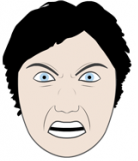
\includegraphics[width=30mm]{./Imagenes/colera.png}
		\caption{Expresión Facial de Cólera}
		\vspace{0.15cm}
		\textit{Fuente: Las 6 emociones básicas, Paul Ekman}
		\label{fig:colera}
\end{figure}}
\end{itemize}}



\item {\textbf{Felicidad:} 
\begin{itemize}
\item \textbf{Descripción.-} Agradable sensación de satisfacción y bienestar.
\item { \textbf{Movimientos musculares faciales.-} Smiling – tirando hacia arriba comisuras de la boca, contrayendo los músculos grandes orbitales alrededor de los ojos.

\begin{figure}[H]
		\centering
		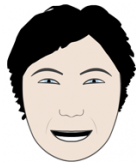
\includegraphics[width=30mm]{./Imagenes/felicidad.png}
		\caption{Expresión Facial de Felicidad}
		\vspace{0.15cm}
		\textit{Fuente: Las 6 emociones básicas, Paul Ekman}
		\label{fig:felicidad}
\end{figure}}
\end{itemize}}



\item {\textbf{Sorpresa:} 
\begin{itemize}
\item \textbf{Descripción.-} Sensación de malestar o sorpresa ante un hecho inesperado.
\item { \textbf{Movimientos musculares faciales.-} Levantando las cejas altas (que puede causar arrugas en la frente), abriendo los ojos como platos, dejando caer la mandíbula tan boca es ágape.

\begin{figure}[H]
		\centering
		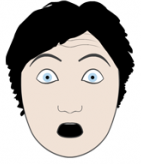
\includegraphics[width=30mm]{./Imagenes/sorpresa.png}
		\caption{Expresión Facial de Sorpresa}
		\vspace{0.15cm}
		\textit{Fuente: Las 6 emociones básicas, Paul Ekman}
		\label{fig:sorpresa}
\end{figure}}
\end{itemize}}


\item {\textbf{Asco:} 
\begin{itemize}
\item \textbf{Descripción.-} Desagrado intenso o condena causada por algo ofensivo o repulsiva.
\item { \textbf{Movimientos musculares faciales.-} La reducción de las cejas, curvando el labio superior, arrugando la nariz.

\begin{figure}[H]
		\centering
		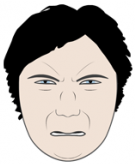
\includegraphics[width=30mm]{./Imagenes/asco.png}
		\caption{Expresión Facial de Asco}
		\vspace{0.15cm}
		\textit{Fuente: Las 6 emociones básicas, Paul Ekman}
		\label{fig:asco}
\end{figure}}
\end{itemize}}



\item {\textbf{Tristeza:} 
\begin{itemize}
\item \textbf{Descripción.-} Sentimiento de infelicidad o tristeza.
\item { \textbf{Movimientos musculares faciales.-} Los párpados caídos, la reducción de las esquinas de la boca, labios fruncidos, los ojos bajos.

\begin{figure}[H]
		\centering
		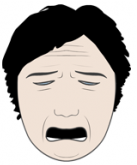
\includegraphics[width=30mm]{./Imagenes/tristeza.png}
		\caption{Expresión Facial de Tristeza}
		\vspace{0.15cm}
		\textit{Fuente: Las 6 emociones básicas, Paul Ekman}
		\label{fig:tristeza}
\end{figure}}
\end{itemize}}


\item {\textbf{Miedo:} 
\begin{itemize}
\item \textbf{Descripción.-} Sensación de aprehensión provocada por la percepción de peligro, amenaza o imposición de dolor.
\item { \textbf{Movimientos musculares faciales.-} Levantando las cejas / dibujar las cejas juntas, tensando los párpados inferiores, que se extiende horizontalmente labios, la boca ligeramente abierta.

\begin{figure}[H]
		\centering
		
\includegraphics[width=30mm]{./Imagenes/miedo.png}
		\caption{Expresión Facial de Miedo}
		\vspace{0.15cm}
		\textit{Fuente: Las 6 emociones básicas, Paul Ekman}
		\label{fig:miedo}
\end{figure}}
\end{itemize}}

\end{itemize}


\subsection{Otras expresiones faciales}
Los hallazgos de Ekman sobre las expresiones faciales universales revelaron el carácter intercultural de la relación entre la comunicación no verbal y la emoción, sin embargo, las teorías de Ekman han evolucionado desde que ideó su lista de emociones básicas. En la década de 1990, añadió una serie de otros a la lista de emociones universales, aunque hizo hincapié en que no todos ellos pueden ser identificados utilizando expresiones faciales. Estas emociones adicionales son~\cite{29ekman2016scientists}

\begin{itemize}
\item Diversión
\item Desprecio
\item Contentamiento
\item Vergüenza	
\item Emoción
\item Culpa
\item El orgullo de los logros
\item Alivio
\item Satisfacción
\item Placer sensorial
\item Vergüenza
\item Neutro
\end{itemize}


\part{Desarrollo del Proyecto}
\chapter{Desarrollo del Detector de Rostros y la Arquitectura de Red Neuronal Convolucional}

\section{Detección de Rostros}
En este trabajo se optó por utilizar como etapa inicial dentro de la fase de consultas a la red, la construcción de un detector de rostros, debido a que, al momento de desarrollar una aplicación orientada a las necesidades del mundo real, este no solo recibira como entrada imágenes que contengan exactamente el rostro de la persona, sino, imágenes con el cuerpo completo o algunas partes adicionales aparte del rostro. Sin embargo, en objetivo del trabajo es poder detectar la expresión facial de una persona, para lo cual, basta con tener como entrada a la red una imagen que delimite el rostro de la persona. De ahí, la necesidad de utilizar un algoritmo de detección de rostros para la extracción de la región de interes que posteriormente servira como entrada para la red neuronal convolucional encargada de reconocer la expresión facial correspondiente. La figura~\ref{fig:imagen_entrada} muestra un ejemplo de una imagen de entrada, en la cual, se puede observar detalles adicionales aparte del rostro(el sombrero y el fondo), los cuales no aportan carasteristicas relevantes que ayuden al reconocimiento de la expresion facial.

Para esta etapa se utilizó el detector de objetos \textit{Haar Cascade}, un algoritmo muy utilizado, cuya implementación puede ser encontrado en distintas librerías orientadas al procesamiento de imágenes, tales como OpenCV\footnote[5]{OpenCV es una librería \textit{open source} que contiene algoritmo relacionados con el area de visión por computador, http://opencv.org/}. Como se describió en la sección~\ref{sec:Haar_Cascade}, este algoritmo utiliza técnicas de \textit{machine learning}. Su proceso de entrenamiento se realiza con imágenes positivas y negativas(imágenes que representan y no representan rostros), creando así un modelo capaz de detectar rostros, basandose en la detecciín de caracteristicas \textit{Haar}. La entrada para esta etapa es una imagen cualquiera, el proceso consiste en detectar el rostro en dicha imagen(en caso exista algun rostro) y extraerlo en otra imagen en escala de grises, la cual tendra un tamaño aproximado de 48x48 pixeles(dependiendo de las dimensiones del rostro). Esta última imagen será la entrada para el modelo en la fase de consultas. Nótese que para la detección de un rostro y la asignación de su respectiva expresión facial, no es necesario mantener la imagen a coloros, puesto que este no es una característica necesaria para conseguir el objetivo. La figura~\ref{fig:proceso_deteccion} muestra los pasos a seguir para la detección y extracción del rostro en una imagen.

\begin{figure}[H]
		\centering
		
\includegraphics[width=50mm]{./Imagenes/imagen_entrada.png}
		\caption{Ejemplo de una imagen de entrada.}
		\vspace{0.15cm}
		\textit{Fuente: Consuelo Ferrús, http://www.acompasando.org/orar-el-asombro/}
		\label{fig:imagen_entrada}
\end{figure}


\begin{figure}[H]
		\centering
		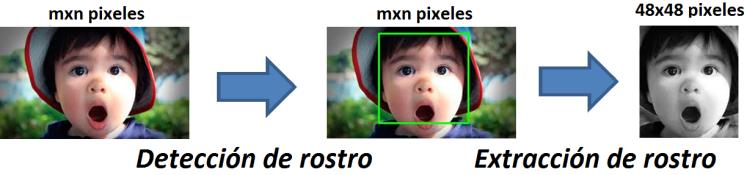
\includegraphics[width=140mm]{./Imagenes/proceso_deteccion.png}
		\caption{Proceso de detección de rostro.}
		\vspace{0.15cm}
		\textit{Fuente: Propio}
		\label{fig:proceso_deteccion}
\end{figure}

Se optó por la utilización del detector de rostros \textit{Haar Cascade}, debido a que este es ampliamente utilizado por el nivel de precisión que posee~\cite{6russakovsky2015imagenet}. Sin embargo, esta técnica aun presenta algunas fallas cuando el rostro presenta algún tipo de oclusión(figura~\ref{fig:oclussion}). Este tipo de problema tambien puede ser solucionado construyendo una red convolucional orientada a la detección o localización de rostros, o por medio de otro tipo de técnicas tradicionales basadas en la extracción de características. Debido al tiempo y bajos recursos computacionales, se opto por proponer este tipo de enfoques como trabajos futuros.

\begin{figure}[H]
		\centering
		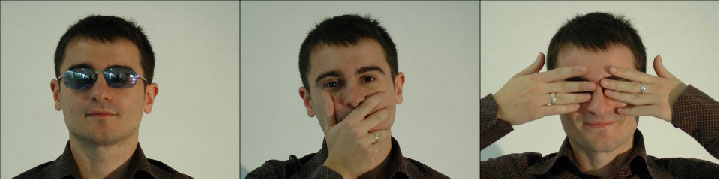
\includegraphics[width=130mm]{./Imagenes/oclussion.jpeg}
		\caption{Ejemplo de rostros con oclusión.}
		\vspace{0.15cm}
		\textit{Fuente: Face Dataset, Universidad Politécnica de Catalunya.}
		\label{fig:oclussion}
\end{figure}

\section{Experimentación en la Elección de Parámetros y Capas en la Construcción de la Arquitectura CNN}
\label{sec:experiment}
La creación de un modelo robusto a partir de la utilización de redes neuronales convolucionales, es una tarea muy complicada, debido a que en la actualidad no existen estudios que indique cual es la configuración correcta que esta debe seguir. Es así, que todos los trabajos que utilizan cualquier técnica perteneciente a \textit{deep learning}, se basan en la experimentación sobre diversar configuraciones en la arquitectura, estas configuraciones estan relacionadas con el numero de capas de convolución, sub-muestreo, totalmente conectadas, tipos de funciones de activacion y normalizacion. Otros elementos muy importantes que tambien son considerados al momento de realizar experimentos, son los parámetros de cada capa, tales como: el número y tamaño de los filtros en la capa de convolucion, operaciones de agrupación en la capa de sub-muestreo, etc.

Sin embargo, entrenar un red neuronal no es una tarea fácil, debido a que se tienen que optimizar miles de parametros para la creación de un buen modelo, asi como las miles de multiplicaciones de matrices que tienen que llevarse a cabo para realizar la operación de convolución. Es así que el número de experimentos que se puedan realizar, depende mucho de la insfraestructura y \textit{hardware} sobre el cual se esta trabajando, siendo este una gran limitante para una extensa experimentación.

Según lo explicado en los parrafos anteriores, para encontrar la correcta configuracion de una arquitectura basada en las redes neuronales convolucionales que resuelva el problema de reconocimiento de expresiones faciales, se realizaron muchos experimentos, cada uno con una configuracion diferente que la anterior. En total se evaluaron 3 arquitecturas con distintas configuracion de capas y parametros, en cada una de estas se calculo la precision y error utilizando las bases de datos FER2013 y CK.




\begin{itemize}
\item {\textbf{Conv-Conv-Pool-Conv-Conv-Pool-FC}

\begin{table}[H]
    \centering
    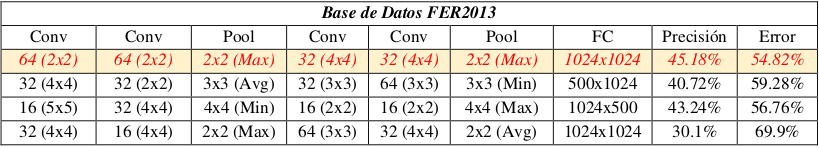
\includegraphics[width=140mm]{./Imagenes/tabla_arqui_1_fer.png} 
    \caption{Evaluación de la arquitectura 1 y sus parámetros, FER2013}
    \label{tab:tabla_arqui_1_fer}
\end{table}

\begin{table}[H]
    \centering
    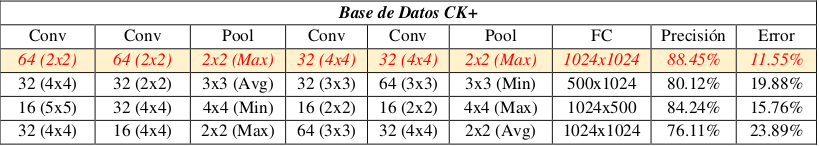
\includegraphics[width=140mm]{./Imagenes/tabla_arqui_1_CK.png}
    \caption{Evaluación de la arquitectura 1 y sus parámetros, CK+}
    \label{tab:tabla_arqui_1_CK}
\end{table}

}

\item {\textbf{Conv-Pool-Conv-Pool-FC \underline{\textit{Arquitectura Propuesta}} }

\begin{table}[H]
    \centering
    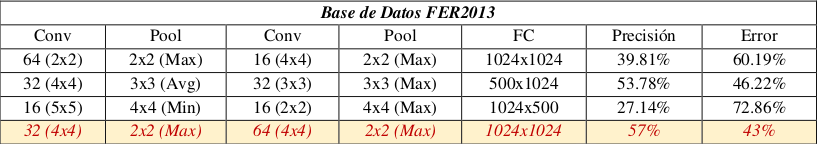
\includegraphics[width=140mm]{./Imagenes/tabla_arqui_2_fer.png} 
    \caption{Evaluación de la arquitectura 2 y sus parámetros, FER2013}
    \label{tab:tabla_arqui_2_fer}
\end{table}

\begin{table}[H]
    \centering
    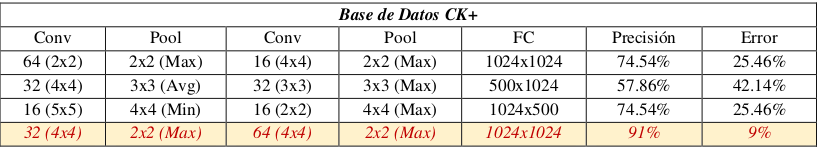
\includegraphics[width=140mm]{./Imagenes/tabla_arqui_2_CK.png}
    \caption{Evaluación de la arquitectura 2 y sus parámetros, CK+}
    \label{tab:tabla_arqui_2_CK}
\end{table}

}

\item {\textbf{Conv-Pool-Pool-Conv-Conv-Pool-FC}

\begin{table}[H]
    \centering
    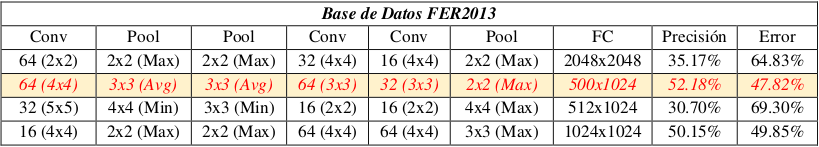
\includegraphics[width=140mm]{./Imagenes/tabla_arqui_3_fer.png} 
    \caption{Evaluación de la arquitectura 3 y sus parámetros, FER2013}
    \label{tab:tabla_arqui_3_fer}
\end{table}

\begin{table}[H]
    \centering
    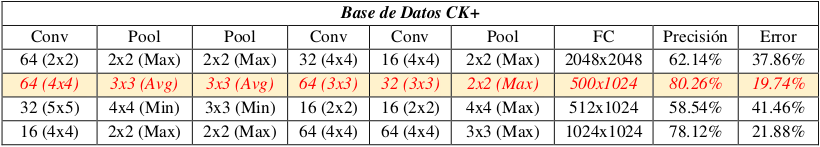
\includegraphics[width=140mm]{./Imagenes/tabla_arqui_3_CK.png}
    \caption{Evaluación de la arquitectura 3 y sus parámetros, CK+}
    \label{tab:tabla_arqui_3_CK}
\end{table}
}
\end{itemize}

De acuerdo con los experimentos realizados, se puede obsevar que la mejor configuracion de capas es: convolucion-\textit{pooling}-convolucion-\textit{pooling}-FC, con 32 y 64 filtros de tamaño 4$\times$4 en la primera y segunda capa de convolucion respectivamente, ventanas de agrupacion de 2$\times$2 en las dos capas de sub-muestreo y un total de 1024$\times$1024 neuronas en las ultimas capas totalmente conectadas.

Segun los resultados mostrados en las tablas~\ref{tab:tabla_arqui_1_fer} y~\ref{tab:tabla_arqui_1_CK} se puede concluir que, la utilización de dos capas consecutivas de convolución es una mala elección, debido a que el hecho de aplicar dos filtros consecutivos hace que la información de la imagen se pierda mas rápidamente que lo normal, ya que el tamaño de la imagen se reduce significativamente después de cada una de estas operaciones. También, las tablas~\ref{tab:tabla_arqui_3_fer} y~\ref{tab:tabla_arqui_3_CK} muestran resultados muy por debajo de la segunda configuración(la mejor obtenida en los experimentos realizados), similar que la explicacion anterior, se concluye que se dan estos resultados debido a la utilizacion de dos capas consecutivas de sub-muestreo, ya que el objetivo de estas capaz es reducir las dimensiones de la imagen solo preservando información reelevante, sin embargo, al realizar una operación de sub-muestreo detras de otra, hace que se pierda mas información de la necesaria. 

\section{Arquitectura Propuesta}
\label{sec:arq_propuesta}
De acuerdo con los experimentados mostrados en la seccion~\ref{sec:experiment}, la arquitectura que consiguio los mejores resultados sigue la siguiente configuracion: la entrada consta de una imagen de 48x48 pixeles en escala de gris, que es el resultado de la fase de detección y extracción de rostro, seguido de una capa de 32 convoluciones con filtro de 4x4 sin solapamiento, luego se aplica un sub muestreo de 2x2 con función MAX \footnote[6]{Función que determina el máximo de n números.} , seguido de una capa de 64 convoluciones con filtros de 2x2 sin solapamiento, para posteriormente aplicar un sub muestreo tambien de dimensiones 2x2 con función MAX, aplicada las convoluciones y sub muestreo se procede a aplicar el Dropout\footnote[7]{Una forma simple de prevenir el \textit{overfitting} en Redes Neuronales..} con 20\%, seguido de dos capas, con 1024 neuronas totalmente conectadas cada una. Finalmente, para la clasificación se aplica la función de normalización Softmax, la cual toma 6 clases, las cuales representar al numero de expresiones a reconocer.
\vspace{0.5cm}
\begin{table}[H]
    \centering
    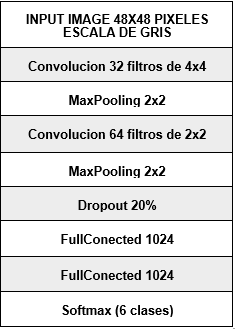
\includegraphics[width=60mm]{./Imagenes/tabla_arquitectura.png}
    \caption{Arquitectura del modelo propuesto}
    \label{tab:tabla_arquitectura}
\end{table}


\begin{figure}[H]
		\centering
		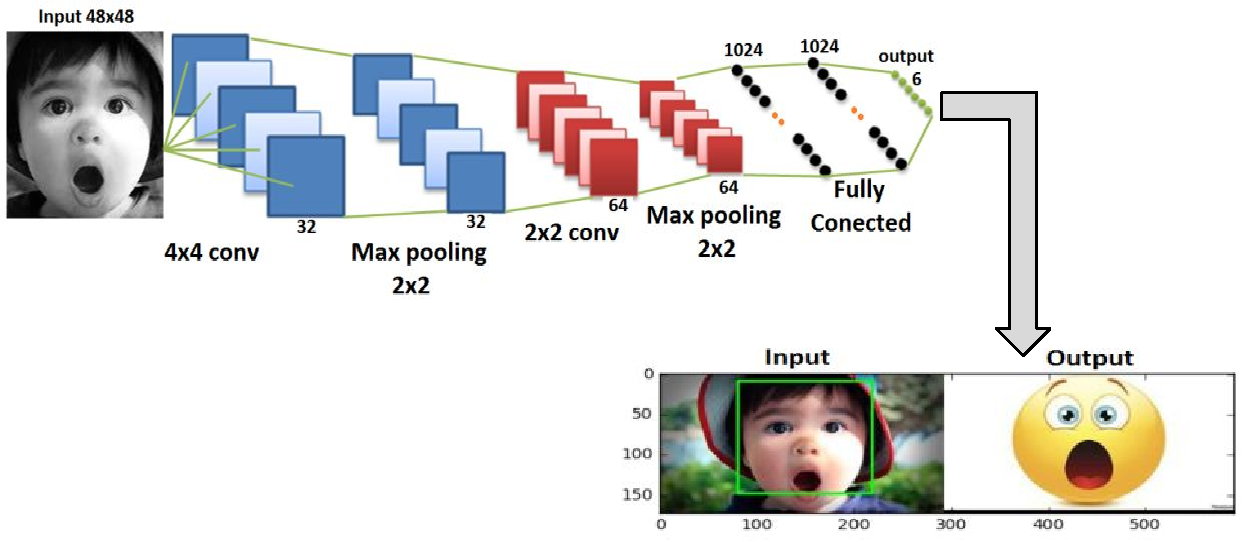
\includegraphics[width=180mm]{./Imagenes/arquitectura_CNN_grafico.pdf}
		\caption{Arquitectura grafica del modelo propuesto.}
		\vspace{0.15cm}
		\textit{Fuente: Propio.}
		\label{fig:arquitectura_CNN_grafico}
\end{figure}

La tabla~\ref{tab:tabla_arquitectura} muestra de arriba para abajo, la representación secuencial de las capas dentro de la arquitectura propuesta antes mencionada. Sin embargo, La figura~\ref{fig:arquitectura_CNN_grafico} muestra de una forma mas detallada cada una de las capas que integran la arquitectura, construyendo de esta forma una red neuronal convolucional. Tambien se muestra en esta figura, la salida final obtenida despues de realizar una consulta sobre el modelo, resaltando el rostro detectado en la imagen de entrada, y relacionando la expresion facial que este tiene con una imagen caricaturizada.

\section{Descripción de la Capas de la Arquitectura}

Dentro de cada capa perteneciente a la red neuronal convolucional, se lleva a cabo operaciones de multiplicacion de matrices, agrupacion de regiones, etc, con el objetivo de extraer o resaltar características importantes de las cuales la red pueda aprender patrones y filtros que se adanten mejor al problema, de tal forma que pueda dar respuestas precisas a entradas futuras. 

Siguiendo el orden de capas de la arquitectura propuestas, presentada en la seccion~\ref{sec:arq_propuesta}, se describe el comportamiento de cada uno de ellos de la siguiente forma: 
\begin{itemize}
\item
{
\textbf{Primera capa convolución.} Cuenta con 32 filtros (mapa de características) de tamaño 4x4 pixeles. Esta capa tiene como objetivo extraer características de alto nivel. La figura~\ref{fig:filtro1} muestra el conjunto de imagenes generadas despues de aplicar los 32 filtros de convolución sobre la imagen de entrada, estas imagenes muestra claramente que en esta capa, la arquitectura se encarga de aprender filtros que sean capaces de extraer bordes y partes fundamentales del rostro, tales como: los ojos, boca, nariz y cejas. Esta primera capa de convolución genera una imagen de salida por cada filtro, siendo así, 32 nuevas imágenes las entradas para la siguiente capa. 

\begin{figure}[H]
		\centering
		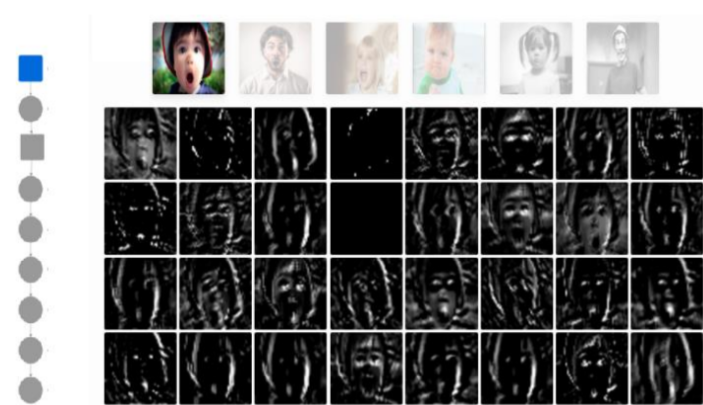
\includegraphics[width=100mm]{./Imagenes/filtro1.png}
		\caption{Imágenes de salida después de la primera convolución.}
		\vspace{0.15cm}
		\textit{Fuente: Propio.}
		\label{fig:filtro1}
\end{figure}
}

\item
{
\textbf{Primera capa de \textit{pooling} o sub-muestreo.} Recibe como parámetros de entrada, las 32 imágenes generadas a partir de la primera capa de convolución. Su función es la de reducir características redundantes mediante la agrupación de pixeles y eleccion del mejor de entre ellos, esta agrupacion se realiza en sub-regiones no solapadas de la matriz, de dimensiones 2$\times$2. Despues de obtener estas sub-regiones, se obtiene el maximo pixel de entre ellas para ser la salida de dicha sub-region. La figura~\ref{fig:filtro2} muestra imágenes semejantes a las obtenidas por la primera capa de convolución, esto se debe a que esta capa no realiza ninguna alteración en el valor de los píxeles, mas al contrario, esta encargada de reducir las dimensiones de las imágenes de entrada, eliminando los píxeles menos significativos. Debido a que se aplica este tipo de operaciones a cada imagen de entrada de esta capa, su número de imágenes de salida sera igual a su numero de entradas.

\begin{figure}[H]
		\centering
		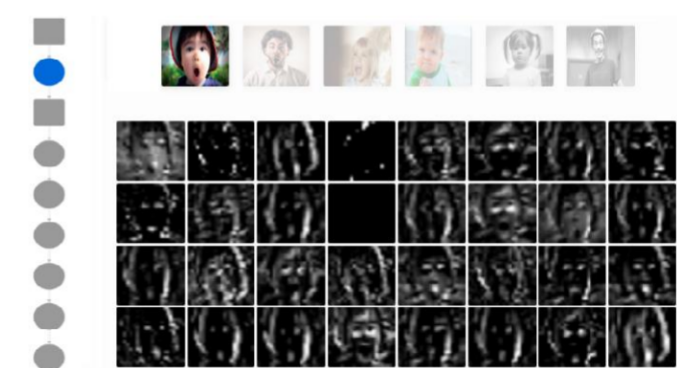
\includegraphics[width=100mm]{./Imagenes/filtro2.png}
		\caption{Imágenes de salida después del primer sub-muestreo.}
		\vspace{0.15cm}
		\textit{Fuente: Propio.}
		\label{fig:filtro2}
\end{figure}
}

\item
{
\textbf{Segunda capa de convolución.} Cuenta con 64 filtros y recibe como parámetros de entrada las imágenes generadas a partir de la primera capa de sub-muestreo. A diferencia de la primera capa de convolución, su funcion es la de extraer y detectar caracteristicas de mas bajo nivel. La figura~\ref{fig:filtro3} muestra las 64 imagenes generadas a partir los filtros de esta capa, en ellas se puede observar de manera mas abstracta ciertos puntos y rectas que representan partes del rostro de la imagen de entrada. Como se menciono anteriormente, esta capa origina 64 imágenes de salida, cada una con un tamaño de 21$\times$21 píxeles.

\begin{figure}[H]
		\centering
		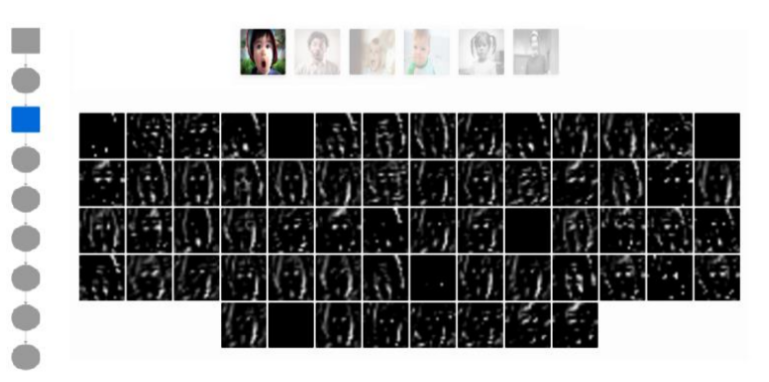
\includegraphics[width=100mm]{./Imagenes/filtro3.png}
		\caption{Imágenes de salida después de la segunda convolución.}
		\vspace{0.15cm}
		\textit{Fuente: Propio.}
		\label{fig:filtro3}
\end{figure}
}

\item
{
\textbf{Segunda capa de \textit{pooling} o sub-muestreo.} Recibe como parámetros de entrada las imágenes generadas a partir de la segunda capa de convolución. Similar que la primera capa de sub-muestreo, es la encargada de eliminar características no relevantes de las imágenes de entrada, mediante la agrupación y selección del mejor píxel, las sub-regiones de agrupacion son de dimensiones 2$\times$2. La figura~\ref{fig:filtro4} muestra las 64 imágenes generadas a partir de esta capa, donde cada una de estas nuevas imágenes son de tamaño 10x10 pixeles. Segun esta figura se puede observar que el rostro se distorsiona y pierde su forma original, siendo estas, a lo que se conoce como características de bajo nivel.
\begin{figure}[H]
		\centering
		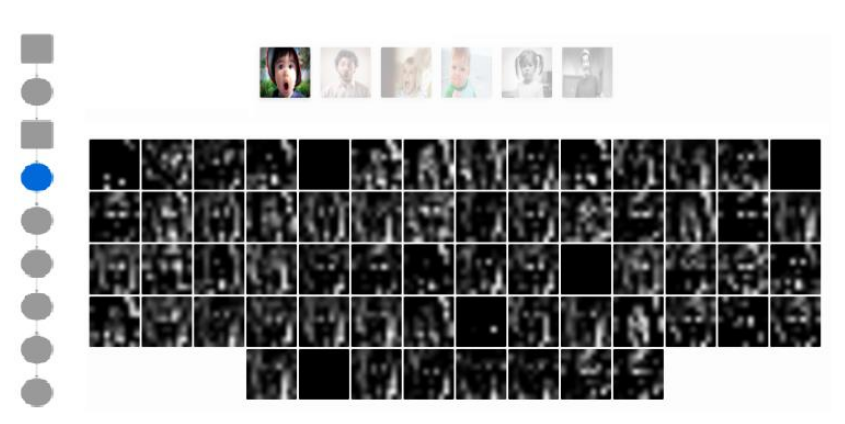
\includegraphics[width=100mm]{./Imagenes/filtro4.png}
		\caption{Imágenes de salida después del segundo sub-muestreo.}
		\vspace{0.15cm}
		\textit{Fuente: Propio.}
		\label{fig:filtro4}
\end{figure}
}
\item
{
\textbf{Capas totalmente conectadas.} Recibe como parámetros de entrada las imágenes generadas a partir de la segunda capa de sub-muestreo, las cuales representan las caracteristicas a bajo nivel pertenecientes a la imagen de entrada original. El objetivo de esta capa, es relacionar cada una de estas características por medio de las 2 capas totalmente conectadas con 1024 neuronas cada una, donde cada neurona es una imagen que representa alguna caracteristica encontrada en las capas anteriores. Al final de la arquitectura, se utiliza la función de normalización \textit{softmax} para generar 6 salidas, donde cada una de ellas representa a una expresion facial. La funcion de normalizacion es la encargada de asignar una probabilidad a cada una de estas salidas, siendo nuestra salida final, aquella que presente la mayor probabilidad.
}
\end{itemize}

\section{PARAMETROS DE LA ARQUITECTURA}
La imágenes de entrada son definidas en el tamaño de 48x48 píxeles como valor
estándar basándonos en el tamaño en el cual están las imágenes de la base de datos
FER2013, el número de convoluciones en la primera capa es de 32 y 64 en la segunda
capa de convolución obteniendo así un total de 32x64 mapas de características, la capa
de Pooling agrupa subregiones de las dimensiones 2x2 píxeles para que no se pierda
mucha información, nosotros optamos por la elección de dos capas totalmente conectadas
de 1024x1024 producto de los resultados obtenidos basándonos en prueba y error , el total
de parámetros obtenidos con la arquitectura propuesta es de:

\begin{itemize}
\item Imagen de entrada: 48x48 píxeles
\item 1ra capa con 32 convoluciones: 544 parámetros
\item 2da capa con 64 convoluciones: 8256 parámetros
\item 1ra capa totalmente conectada: 6554624 parámetros
\item 2da capa totalmente conectada: 1049600 parámetros
\item función de normalización Softmax: 7175 parámetros
\end{itemize}
Obteniendo un total de 7,620,199 parámetros totales.

\begin{table}[H]
    \centering
    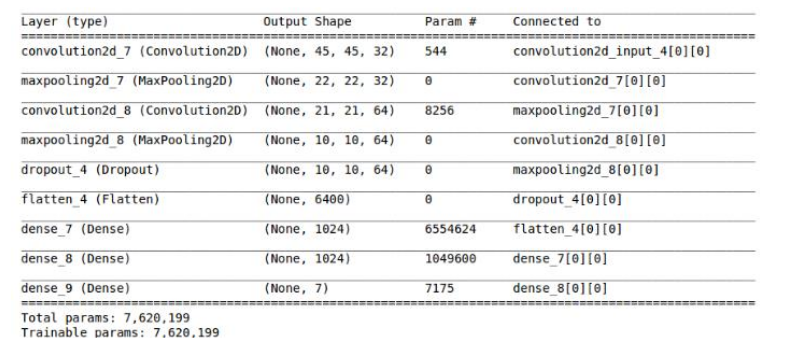
\includegraphics[width=140mm]{./Imagenes/parametros.png} 
    \caption{Número de parámetros de nuestra CNN}
    \label{tab:parametros}
\end{table}

	
\section{ENTRENAMIENDO DE LA CNN}
El entrenamiento de nuestra Red Neuronal Convolucional siguió un proceso
iterativo en el que se presentó como datos de entrada imágenes de expresiones faciales y
sus respectivas etiquetas de salida (clases correspondientes a la expresión facial a la cual
pertenece: enojo, miedo, alegría, tristeza, sorpresa y neutro).

Durante esta fase de entrenamiento, la Red Neuronal Convolucional aprendió
mediante el ajuste de sus pesos, con el fin de ser capaz de predecir la etiqueta de clase
correcta de los datos de entrada, el algoritmo de Red Neuronal más popular para la fase
de entrenamiento es el algoritmo de BackPropagation, dicho algoritmo se usó en nuestra
fase de entrenamiento. Los pesos iniciales de nuestra red se eligieron al azar y comienza
el entrenamiento o aprendizaje. Se procesó los datos de entrada para lograr obtener las
etiquetas deseadas obteniendo un error el cual se propago hacia atrás mediante el
algoritmo antes mencionado(BackPropagation) haciendo que se ajusten los pesos, este
proceso ocurrió una y otra vez hasta que se minimizo el error y eso ocurrió cuando se
logró una convergencia de los datos.

\section{TEST AL MODELO CREADO}
Una vez creada el modelo (un archivo con extensión .h5) se procede a realizar las
consultas a dicho modelo, estas consultas siguen los siguientes pasos:

\begin{itemize}
\item Leer una imagen de entrada, de dimensiones mayos o igual a 48x48 pixeles.
\item Utilizar Haar Cascade para la detección del rostro en la imagen antes ingresado.
\item Extraer el rostro detectado y redimensionarlo al tamaño 48x48 pixeles.
\item Dar como imagen de entrada la imagen obtenida en el paso anterior.
\end{itemize}
Después de realizar los pasos anteriores, el modelo arrojara un valor asociado a la
expresión facial predicha.

\section{RECOPILACIÓN DE IMAGENES DE EXPRESIONES
FACIALES}
La recopilación de las imágenes de expresiones faciales se obtuvo de 2 fuentes
secundarias de información (internet) en los cuales los datos están pre-elaborados
(imágenes con tamaños de 48x48 pixeles de base de datos FER20131 y 640x490 o
640x480 píxeles de la base de datos CK+).

\section{BASE DE DATOS}
Se usó 3 bases de datos ($FER2013^{1}$ y $CK+^{2}$ ) y una tercera como resultado de la
unión de las 2 bases de datos antes mencionadas.
\subsection{FER2013}
Es una base de datos del sitio web Kaggle{1} para el concurso de reconocimiento de
expresiones faciales.

Esta base de datos posee 35887 imágenes en escala de gris de 48x48 pixeles,
clasificados en 7 categorías (enojado, disgustado, miedo, feliz, triste, sorpresa y neutro).
En este trabajo se optó por unir la categoría enojado y disgustado por las similitudes que
tienen entre ellas.

Separamos la data en 2 partes training y test. El training consta de 32298 imágenes
y el test de 3589 imágenes.

\begin{figure}[H]
		\centering
		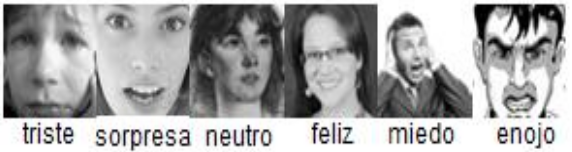
\includegraphics[width=90mm]{./Imagenes/imagenes_fer.png}
		\caption{Imágenes de la base de datos FER2013}
		Source: Kaggle
		\label{fig:imagenes_fer}
\end{figure}

\section{CK+}
La base de datos $CK+^{2}$ (Cohn-Kanade) posee imágenes de expresiones faciales
frontales de 210 personas en resolución de 640x490 o 640x480 pixeles. Nosotros
elegimos de entre ellos 3289 imágenes convirtiéndolos a escala de gris de 48x48 pixeles
y clasificándolos en 6 categorías (enojado, miedo, feliz, triste, sorprendido y neutro).
Nuestro training consta de 2966 imágenes y el test de 323 imágenes.

\begin{figure}[H]
		\centering
		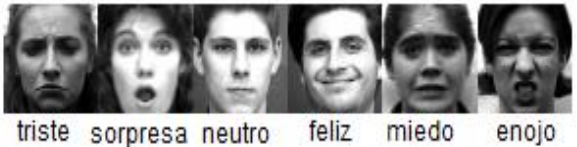
\includegraphics[width=90mm]{./Imagenes/imagenes_ck+.png}
		\caption{Imágenes de la base de datos CK+}
		Source: Base de datos CK+
		\label{fig:imagenes_ck+}
\end{figure}


\section{FER2013 - CK+}
Esta base de datos resulta de la unión de la base de datos Fer2013 y CK+,
obteniendo un total de 39176 imágenes de 48x48 en escala de gris. El training tiene 35264
y el test 3912 imágenes.

\section{RESULTADOS EXPERIMENTALES}
A continuación, se muestra los resultados que se obtuvieron en las diferentes bases
de datos FER2013, CK+ y la tercera base de datos que se obtuvo como resultado de la
unión de los dos antes mencionadas.

Se podrá apreciar los niveles de precisión alcanzado por cada categoría –
Expresión Facial (Enojado, Miedo, Feliz, Triste, Sorprendido, Neutro). Así como sus
matrices de confusión que nos mostraran los resultados positivos y sus falsos positivos,
pudiendo así interpretar de mejor manera los resultados.

\subsection{FER2013}

\begin{table}[H]
    \centering
    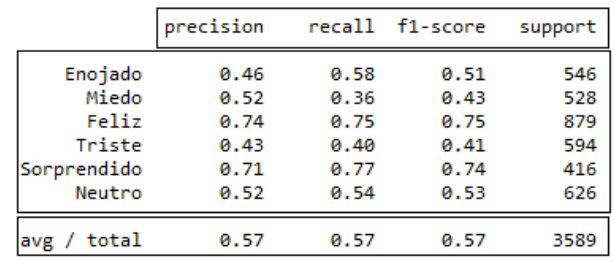
\includegraphics[width=80mm]{./Imagenes/tabla_resultados_fer.png} 
    \caption{Resultados obtenidos - FER2013}
    \label{tab:tabla_resultados_fer}
\end{table}

En la Tabla 3 se puede apreciar los niveles de precisión en la clasificación de los
datos de la base de datos FER2013, mostrando en la categoría Enojado 46\%, Miedo 52\%,
Feliz 74\% Triste 43\%, Sorprendido 71\% y Neutro 52\%.

\begin{figure}[H]
		\centering
		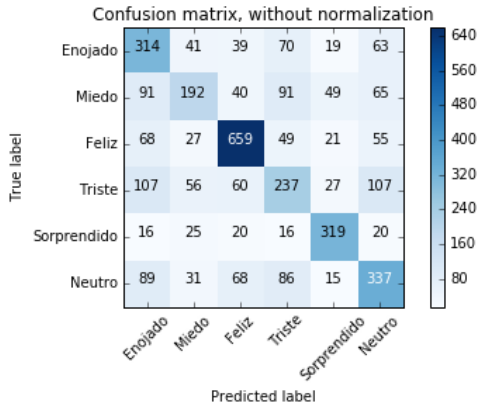
\includegraphics[width=80mm]{./Imagenes/matriz_confusion_fer.png}
		\caption{Matriz de confusión, precisión del Test - FER2013}
		\label{fig:matriz_confusion_fer}
\end{figure}

\begin{figure}[H]
		\centering
		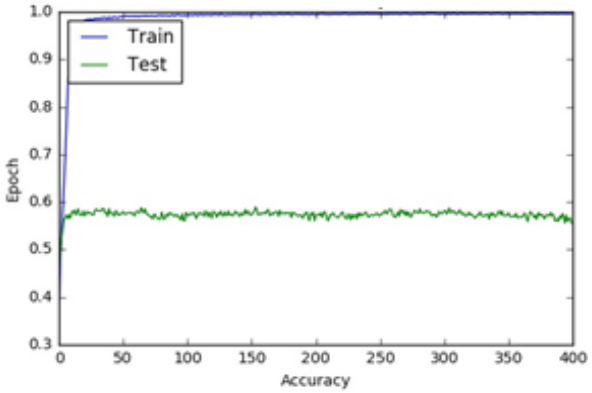
\includegraphics[width=80mm]{./Imagenes/precision_fer.png}
		\caption{Precisión durante el proceso de entrenamiento y prueba (\%) – FER2013}
		\label{fig:precision_fer}
\end{figure}

\begin{figure}[H]
		\centering
		\includegraphics[width=80mm]{./Imagenes/perdida_fer.png}
		\caption{Perdida durante el proceso de entrenamiento y prueba (\%) – FER2013}
		\label{fig:perdida_fer}
\end{figure}

\subsection{CK+}

\begin{table}[H]
    \centering
    \includegraphics[width=80mm]{./Imagenes/tabla_resultados_ck+.png} 
    \caption{Resultados obtenidos - CK+}
    \label{tab:tabla_resultados_ck+}
\end{table}

En la Tabla 4 se puede apreciar los niveles de precisión en la clasificación de los
datos de la base de datos CK+, mostrando en la categoría Enojado 91\%, Miedo 76\%,
Feliz 100\%, Triste 87\%, Sorprendido 100\% y Neutro 78\%.

\begin{figure}[H]
		\centering
		\includegraphics[width=80mm]{./Imagenes/matriz_confusion_ck+.png}
		\caption{Matriz de confusión, precisión del Test - CK+}
		\label{fig:matriz_confusion_ck+}
\end{figure}

\begin{figure}[H]
		\centering
		\includegraphics[width=80mm]{./Imagenes/precision_ck+.png}
		\caption{Precisión durante el proceso de entrenamiento y prueba (\%) - CK+}
		\label{fig:precision-ck+}
\end{figure}

\begin{figure}[H]
		\centering
		\includegraphics[width=80mm]{./Imagenes/perdida_ck+.png}
		\caption{Perdida durante el proceso de entrenamiento y prueba (\%) – FER2013}
		\label{fig:perdida_ck+}
\end{figure}

\subsection{FER2013 - CK+}


\begin{table}[H]
    \centering
    \includegraphics[width=80mm]{./Imagenes/tabla_resultados_fer_ck+.png} 
    \caption{Resultados obtenidos - FER2013 - CK+}
    \label{tab:tabla_resultados_fer_ck+}
\end{table}

En la Tabla 5 se puede apreciar los niveles de precisión en la clasificación de los
datos de la base de datos (FER2013 - CK+), mostrando en la categoría Enojado 57\%,
Miedo 48\%, Feliz 75\%, Triste 44\%, Sorprendido 77\% y Neutro 53\%

\begin{figure}[H]
		\centering
		\includegraphics[width=80mm]{./Imagenes/matriz_confusion_fer_ck+.png}
		\caption{Matriz de confusión, precisión del Test FER2013 - CK+}
		\label{fig:matriz_confusion_fer_ck+}
\end{figure}

\begin{figure}[H]
		\centering
		\includegraphics[width=80mm]{./Imagenes/precision_fer_ck+.png}
		\caption{Precisión durante el proceso de entrenamiento y prueba (\%) FER2013 - CK+}
		\label{fig:precision_fer_ck+}
\end{figure}

\begin{figure}[H]
		\centering
		\includegraphics[width=80mm]{./Imagenes/perdida_fer_ck+.png}
		\caption{Perdida durante el proceso de entrenamiento y prueba (\%) FER2013 - CK+}
		\label{fig:perdida_fer_ck+}
\end{figure}





\chapter*{Resultados Generales}

Se obtuvo un nivel de precisión de 91\% en los experimentos realizados con la base de datos CK+ (sub-seccion~\ref{subsec:ck+}), 57\% con FER2013 (sub-seccion~\ref{subsec:fer2013}) y 60\% con la unión de ambas bases de datos (sub-seccion~\ref{subsec:ck+fer2013}), estando 14\% debajo del nivel de precisión del primer lugar del concurso mundial de reconocimiento de expresiones faciales organizado por \textit{Kaggle} (utilizando la base de datos FER2013). Se presume que dichos resultados no alcanzaron ni superaron métodos del estado del arte, debido a la cantidad de experimentos realizados por las limitaciones de Hardware que se presentaron en el desarrollo de este trabajo (uso de CPU más no de GPU en la fase de entrenamiento). Sin embargo, los resultados obtenidos con la base de datos CK+ son prometedores, debido a la variedad de imágenes de expresiones faciales  que este conjunto de datos posee.

\renewcommand\bibname{Resultados}
\addcontentsline{toc}{chapter}{Resultados}
\chapter*{CONCLUSIONES}
\begin{itemize}

\item En este trabajo, desarrollamos un clasificador para el reconocimiento de expresiones faciales considerando seis categorías (alegre, neutro, feliz, triste, enojado, sorpresa).

\item Las bases de datos usadas en este trabajo Fer2013 \ref{subsec:fer2013} y CK+ \ref{subsec:ck+}, fueron estandarizados en tamaño y posteriormente normalizados en valor para reducir la varianza en los datos. 

\item Adicionalmente, se creo una tercera base de datos llamado Fer2013-CK+ \ref{subsec:ck+fer2013}, como resultado de la unión de las bases de datos Fer2013 y CK+.  

\item Desarrollamos una arquitectura de red neuronal convolucional para el reconocimiento de expresiones faciales \ref{sec:arq_propuesta}.

\item La arquitectura usada para crear el modelo para el reconocimiento de expresiones faciales fue el resultado de tres arquitecturas propuestas, siendo seleccionada la arquitectura con mejores resultados en los experimentos \ref{sec:experiment}.

\item Cada una de las tres arquitectura propuestas, tuvo una  configuración diferente de los elementos principales que componen una red neuronal convolucional (número de capas de convolución, tamaño de los filtros de convolución, número de capas de pooling, operación de pooling, número de capas de neuronas totalmente conectadas, número de neuronas en la capa totalmente conectada) basada en trabajos de la literatura de \textit{deep learning} mostrados en \ref{sec:experiment}..

\item Se realizó satisfactoriamente los experimentos en las tres bases de datos utilizadas Fer2013, CK+ y Fer2013-CK+ \ref{sec:experiment}.

\item Se evaluó los resultados obtenidos por el modelo creado en las tres bases de datos Fer2013, CK+, Fer2013-CK+. Obteniendo un resultado de 90 \% de precisión en la base de datos CK+, mientras que en las bases de datos Fer2013 y Fer2013-CK+ se obtuvo 57\% y 60\% de precisión respectivamente (más detalles ver Tablas ~\ref{tab:tabla_resultados_ck+}, ~\ref{tab:tabla_resultados_fer}, ~\ref{tab:tabla_resultados_fer_ck+} ).


\item Adicionalmente, se tenía la idea de alterar las imagenes de los conjuntos de datos con rotaciones variadas, iluminación, etc (imágenes sintéticas). Sin embargo, esto no representaría las condiciones de las imágenes del mundo real, por lo que nosotros optamos por recolectar un pequeño conjunto de imágenes de internet con contenido variado (fondo con diferente iluminación, oclusión parcial del rostro, posición rotada en algunos rostros, imagen de animes) que si representan en su mayoria las condiciones de las imágenes del mundo real. Así, se  hicieron pruebas en este conjunto de imágenes de internet. Los resultados obtenidos (pruebas satisfactorias - pruebas fallidas) son mostrados en \ref{sec:testing}.

\end{itemize}
\renewcommand\bibname{Conclusiones}
\addcontentsline{toc}{chapter}{Conclusiones}
\chapter*{RECOMENDACIONES}

Por la experiencia en la realización el presento proyecto de investigación, se
recomienda:

\begin{itemize}
\item Desarrollar la fase de entrenamiento con una CPU con capacidad mínima de 8GB
de RAM, y en caso se cuente con la posibilidad de obtener una GPU, como
mínimo esta debe tener 4GB.

\item Acceder a material de investigación (papers. artículos científicos y otros) de
instituciones prestigiosas como la IEEE, ACM, SPRINGER y otros.

\item Usar Python como lenguaje de programación por las facilidades que brinda y por
el uso concurrido a nivel mundial.

\item Asistir a congresos de Machine Learning y Pattern Recognition para poder
resolver dudas existentes directamente con expertos en esta área de investigación.

\end{itemize}
\renewcommand\bibname{Recomendaciones}
\addcontentsline{toc}{chapter}{Recomendaciones}
\chapter*{TRABAJOS FUTUROS}

En este trabajo se abordo el reconocimiento de expresiones en imágenes estáticas por medio de redes neuronales convolucionales. Por lo que se tiene pendiente como trabajos futuros la realización de un clasificador de expresiones faciales en tiempo real. Para lo cual tenemos pensado en la utilización de técnicas mas avanzadas para la fase de detección de rostros. Redefinir la arquitectura propuesta para una arquitectura mas profunda. así, como la útilización técnicas de de \textit{data augmentation} para incrementar la base de datos y aumentar la variabilidad de las imágenes y \textit{transfer learning} mejorar el modelo en la fase de entrenamiento.


\renewcommand\bibname{TrabajosFuturos}
\addcontentsline{toc}{chapter}{Trabajos Futuros}

\end{spacing}


%----------------------bibliografia

%\cleardoublepage
\addcontentsline{toc}{chapter}{Bibliografía}
\begin{spacing}{1.0}
\nocite{*}
\bibliographystyle{abbrv} % estilo de la bibliografía.
\bibliography{bibli.bib} % yyyy.bib es el fichero donde está salvada la bibliografía.

\end{spacing}


%----------------------------------apendix

\appendix

\part*{ANEXOS}
\addcontentsline{toc}{chapter}{ANEXOS}

\chapter{OTROS CONCEPTOS}\label{A}
\section{Matriz de Confusión}

La matriz de confusion es una técnica que facilita el análisis del rendimiento de un algoritmo de clasificación. Frecuentemente, el rendimiento de un clasificador es solo analizado en términos de \textit{precision} (verdaderos positivos, verdaderos negativos y falsos positivos). Sin embargo, este no refleja completamente el verdadero rendimiento del clasificador. Así, comunmente es considerado el \textit{recall} para solucionar parcialmente este problema. El \textit{recall} toma en cuenta los falsos negativos (repuestas predichas como falsas cuando en realidad son verdaderas). Adicionalmente, para evaluar el rendimiento final de un clasificador en forma completa se usa el \textit{f1-score}. El f1-score toma en consideración tanto \textit{precision} y el \textit{recall}, obtiendo una penalización del rendimiento del clasificador cada vez que este se equivoque \cite{30Mconfusion}.
Así, la matriz de confusión cumple un papel importante en el calculo de \textit{precision}, \textit{recall} y \textit{f1-score}. En la Tabla \ref{tab:estruc_confusion_matrix} se puede observar la estructura general de una  matriz de confusión. así mismo en las ecuaciones \ref{eq:Aprecision} y \ref{eq:Arecall}  se muestra el uso de los elementos la matriz de confusión para calcular las métricas de \textit{precision} y \textit{recall} respectivamente. Finalmente, la ecuación \ref{eq:Af1score} muestra el cálculo de \textit{f1-score}. 


\begin{table}[!htb]
  
  \noindent
  \renewcommand\arraystretch{1.5}
  \setlength\tabcolsep{0pt}
  \begin{center}
  \begin{tabular}{c >{\bfseries}r @{\hspace{0.7em}}c @{\hspace{0.4em}}c @{\hspace{0.7em}}l}
    \multirow{10}{*}{\rotatebox{90}{\parbox{1.1cm}  { \bfseries\centering  Valores \\ predichos}}} & 
      & \multicolumn{2}{c}{\bfseries Valores referenciales} & \\
    & & \bfseries Positivos & \bfseries Negativos \\
    & {Predichos positivos} & \MyBox{True}{Positive (TP)} & \MyBox{False}{Negative (FN)} \\[2.4em]
    & Predichos negativos & \MyBox{False}{Positive (FP)} & \MyBox{True}{Negative (TN)} \\
  
  \end{tabular}
  \end{center}
    \caption{Estructura general de la matriz de confusión}
        \label{tab:estruc_confusion_matrix}
\end{table}

\begin{equation}\label{eq:Aprecision}
precision = \frac{ TP}{TP+FP}
\end{equation}

\begin{equation}\label{eq:Arecall}
recall = \frac{ TP}{TP+FN}
\end{equation}

\begin{equation}\label{eq:Af1score}
f1-score = \frac{2 \cdot precision\cdot recall}{precision+ recall}
\end{equation}



\section{Machine Learning}
A grandes rasgos se puede decir que el Machine Learning o aprendizaje
automático es un tipo de Inteligencia Artificial dirigido al desarrollo de técnicas para que
las máquinas puedan aprender y tomar decisiones por sí mismas.
Este aprendizaje es posible gracias a la detección de patrones dentro de un
conjunto de datos de manera que es el propio programa el que predice qué situaciones
podrían darse o no. Estos cálculos son los que les permiten aprender para, finalmente,
generar decisiones y resultados fiables \cite{31MLApplications}.

\section{Aplicaciones de Machine Learning}
El aprendizaje automático cuenta con tantas aplicaciones como imaginemos,
pudiéndose adaptar a tantas situaciones como datos con los que contemos. Motores de
búsqueda, diagnósticos médicos, reconocimiento del habla y del lenguaje, robótica, entre
otras, éstas son algunas de las actividades de nuestro día a día que se ven impulsadas por
el \textit{machine learning} \cite{31MLApplications}:


\begin{itemize}
\item Detección de rostro. Podemos verlo en nuestras cámaras móviles.
\item Reconocimiento facial, de voz o de objetos.
\item 	Buscadores. Para mejorar los resultados y sugerencias de búsqueda.
\item Anti-spam. Mediante el uso de etiquetas.
\item Anti-virus. Para la detección de software malicioso.
\item Genética. Por ejemplo, en la clasificación de secuencias de ADN.

\item Predicción y pronósticos del clima, tráfico o para evitar fallos tecnológicos en
equipos.

\item Comprensión de textos. Se aplica a resúmenes estructurados de noticias o
comentarios sobre un tema específico.

\item Vehículos autónomos y robots.

\item Métodos de optimización más rápidos y flexibles. Se evalúa qué momento es el
adecuado para una tarea concreta.

\item Análisis de imágenes de alta calidad.

\item Análisis de datos económicos para operar en el mercado de valores o evitar el
fraude en transacciones.

\item Análisis de comportamiento de consumo y productividad. Para la identificación
de clientes potenciales, prever qué empleados pueden ser más rentables, adaptar
servicios a las necesidades del usuario y otros

\end{itemize}


\section{Early Stopping}

Durante el entrenamiento de redes neuronales, numerosas decisiones tienen que
ser tomadas con respecto a los ajustes (hiperparámetro) utilizados, con el fin de obtener
un buen rendimiento. Tales hiperparámetro son el número de epoch de formación: es
decir, el número de veces que utilizaremos el conjunto de datos. Si utilizamos muy pocas
épocas, podríamos ocasionar \textit{underfit} (es decir, no aprende todo lo que podamos de los
datos de entrenamiento); si usamos demasiadas epoch, podríamos ocasionar un \textit{overfit} (es decir, colocar el "ruido" en los datos de entrenamiento, y no la señal).

Early Stopping intenta eliminar la necesidad de configurar manualmente este
valor. También se puede considerar un tipo de método de regularización (como L1 / L2
y el dropout) en que se puede detener la red de \textit{overfitting}. 

La idea detrás de Early Stopping es relativamente simple \cite{32Stopping}:


\begin{itemize}
 \item Los datos están divididos en training y test.
 \item Al final de cada epoch (o, cada N epoch):
  \begin{itemize}
  \item Evaluar el rendimiento de la red en el equipo de prueba
  \item Si la red supera al mejor modelo anterior: guardar una copia de la red en
  la epoch actual
  \end{itemize}
  \item Tomar como modelo final el modelo que tiene el mejor rendimiento del test
  Esto se muestra gráficamente a continuación
\end{itemize}


\begin{figure}[!htb]
    \centering
    \includegraphics[width=100mm]{Imagenes/early_stopping.png}
    \caption{Representación gráfica deEarly Stopping}
    \label{fig:early_stopping}
    
\end{figure}




\chapter{TESTING}
\section{Pruebas satisfactorias}
\begin{frame}

\begin{figure}[!htbp]
    
    \begin{multicols}{2}
     \includegraphics[angle=0,width=48mm]{Imagenes/test1.png}
       \caption{Test 1}
       \label{fig:test1}   
       
       \includegraphics[angle=0,width=55mm]{Imagenes/test2.png}
           \caption{Test 2}
           \label{fig:test2} 
           
    \end{multicols}
        
\end{figure}
\end{frame}


\begin{frame}

\begin{figure}[!htbp]
    
    \begin{multicols}{2}
     \includegraphics[angle=0,width=50mm]{Imagenes/test3.png}
       \caption{Test 3}
       \label{fig:test3}   
       
       \includegraphics[angle=0,width=50mm]{Imagenes/test4.png}
           \caption{Test 4}
           \label{fig:test4} 

           
            \includegraphics[angle=0,width=50mm]{Imagenes/test5.png}
              \caption{Test 5}
              \label{fig:test5}   
              
              \includegraphics[angle=0,width=50mm]{Imagenes/test6.png}
                  \caption{Test 6}
                  \label{fig:test6}   
                  
                  
    \end{multicols}
        
\end{figure}
\end{frame}


\begin{frame}

\begin{figure}[!htbp]

   \centering
\includegraphics[angle=0,width=50mm]{Imagenes/test7.png}
    \caption{Test 7}
    \label{fig:test7} 

        
\end{figure}
\end{frame}



 
\section{Pruebas Fallidas}
\begin{frame}

\begin{figure}[!htbp]
    
    \begin{multicols}{2}
     \includegraphics[angle=0,width=48mm]{Imagenes/test8.png}
       \caption{Test 8}
       \label{fig:test8}   
       
       \includegraphics[angle=0,width=55mm]{Imagenes/test9.png}
           \caption{Test 9}
           \label{fig:test9} 
           
    \end{multicols}
        
\end{figure}
\end{frame}




\chapter{HERRAMIENTAS}
Las herramientas de software y hardware son:

\section{Software}
\begin{itemize}
 \item Sistema Operativo. Linux 14.0
 \item Lenguaje de programacion: Python 2.7
 \item Framework Deep Learning: Keras
\end{itemize}

\section{Hardware}
\begin{itemize}
 \item CPU: Intel XEON 3.4 GHz
 \item RAM: 8GB
\end{itemize}

\chapter{GLOSARIO}
\begin{itemize}
\item \textbf{Convolución:} Operador matemático que transforma 2 funciones en una tercera función.
\item \textbf{Modelo:} Representación abstracta, conceptual, gráfica, física o matemática, de
fenomenos, sistemas o procesos a fin de analizarlos, describirlos, explicarlos, simularlos
y predecirlos.
\item \textbf{Arquitectura}: Técnica y estilo con lo que se diseña, proyecta y construye un modelo.
\item 
\textbf{Gradiente:} Derivada parcial de una funcion respecto a cada variable de está.

\item \textbf{Exabyte:} Unidad de medida de almacenamiento de datos cuyo símbolo es el 'EB' equivalente a $10^18$ bytes.

\item \textbf{Kaggle:} Plataforma online que ofrece a sus usuarios la opción de participar en distintas
competencias cuyo principal tema es el análisis de gran cantidad de datos.


\item \textbf{Deep Learning} (DL), es un conjunto de algoritmos en aprendizaje automático que intenta
modelar abstracciones de alto nivel en datos usando arquitecturas compuestas de
transformaciones no-lineales múltiples.



\item \textbf{Convolutional Neural Network} (CNN) , tipo de red neuronal artificial donde las neuronas
corresponden a campos receptivos de una manera muy similar a las neuronas en la corteza
visual primaria de un cerebro biológico.

\item \textbf{Machine Learning} (ML) , es una rama de la inteligencia artificial cuyo objetivo es
desarrollar técnicas que permitan a las computadoras aprender.


\item \textbf{Red Neuronal Artificial} (RNA), modelos matemáticos, computacionales, artificiales,
ideales de una red neuronal empleados en estadística, psicología cognitiva, e inteligencia
artificial.


\item \textbf{ Graphics Processor Unit} (GPU), es un coprocesador dedicado al procesamiento de
gráficos u operaciones de coma flotante, para aligerar la carga de trabajo del procesador
central.

\item \textbf{ImageNet:} Base de datos de imágenes a gran escala con 1.2M de imágenes.


\end{itemize}

\chapter{ACRÓNIMOS}
\begin{itemize}


\item \textbf{ACM:} Association for Computing Machinery, es una sociedad científica y educativa en
ciencias de la computación.

\item \textbf{Mm:} Milímetro, medida de longitud que es igual a la milésima parte de un metro.

\item \textbf{IEEE:} Institute of Electrical and Electronics Engineers, es la mayor organización
profesional técnica del mundo dedicada al avance de la tecnología en beneficio de la
humanidad

\item \textbf{CVPR:} Conference on Computer Vision and Pattern Recognition.

\item \textbf{VLSI:} Sigla en inglés de Very Large Scale Integration

\end{itemize}

%-------------------------------

\end{document}
